\documentclass[]{book}
\usepackage{lmodern}
\usepackage{amssymb,amsmath}
\usepackage{ifxetex,ifluatex}
\usepackage{fixltx2e} % provides \textsubscript
\ifnum 0\ifxetex 1\fi\ifluatex 1\fi=0 % if pdftex
  \usepackage[T1]{fontenc}
  \usepackage[utf8]{inputenc}
\else % if luatex or xelatex
  \ifxetex
    \usepackage{mathspec}
  \else
    \usepackage{fontspec}
  \fi
  \defaultfontfeatures{Ligatures=TeX,Scale=MatchLowercase}
\fi
% use upquote if available, for straight quotes in verbatim environments
\IfFileExists{upquote.sty}{\usepackage{upquote}}{}
% use microtype if available
\IfFileExists{microtype.sty}{%
\usepackage{microtype}
\UseMicrotypeSet[protrusion]{basicmath} % disable protrusion for tt fonts
}{}
\usepackage[margin=1in]{geometry}
\usepackage{hyperref}
\hypersetup{unicode=true,
            pdftitle={Probability and Genetics},
            pdfauthor={Bill Bynum and Brian Avery},
            pdfborder={0 0 0},
            breaklinks=true}
\urlstyle{same}  % don't use monospace font for urls
\usepackage{natbib}
\bibliographystyle{apalike}
\usepackage{color}
\usepackage{fancyvrb}
\newcommand{\VerbBar}{|}
\newcommand{\VERB}{\Verb[commandchars=\\\{\}]}
\DefineVerbatimEnvironment{Highlighting}{Verbatim}{commandchars=\\\{\}}
% Add ',fontsize=\small' for more characters per line
\usepackage{framed}
\definecolor{shadecolor}{RGB}{248,248,248}
\newenvironment{Shaded}{\begin{snugshade}}{\end{snugshade}}
\newcommand{\KeywordTok}[1]{\textcolor[rgb]{0.13,0.29,0.53}{\textbf{#1}}}
\newcommand{\DataTypeTok}[1]{\textcolor[rgb]{0.13,0.29,0.53}{#1}}
\newcommand{\DecValTok}[1]{\textcolor[rgb]{0.00,0.00,0.81}{#1}}
\newcommand{\BaseNTok}[1]{\textcolor[rgb]{0.00,0.00,0.81}{#1}}
\newcommand{\FloatTok}[1]{\textcolor[rgb]{0.00,0.00,0.81}{#1}}
\newcommand{\ConstantTok}[1]{\textcolor[rgb]{0.00,0.00,0.00}{#1}}
\newcommand{\CharTok}[1]{\textcolor[rgb]{0.31,0.60,0.02}{#1}}
\newcommand{\SpecialCharTok}[1]{\textcolor[rgb]{0.00,0.00,0.00}{#1}}
\newcommand{\StringTok}[1]{\textcolor[rgb]{0.31,0.60,0.02}{#1}}
\newcommand{\VerbatimStringTok}[1]{\textcolor[rgb]{0.31,0.60,0.02}{#1}}
\newcommand{\SpecialStringTok}[1]{\textcolor[rgb]{0.31,0.60,0.02}{#1}}
\newcommand{\ImportTok}[1]{#1}
\newcommand{\CommentTok}[1]{\textcolor[rgb]{0.56,0.35,0.01}{\textit{#1}}}
\newcommand{\DocumentationTok}[1]{\textcolor[rgb]{0.56,0.35,0.01}{\textbf{\textit{#1}}}}
\newcommand{\AnnotationTok}[1]{\textcolor[rgb]{0.56,0.35,0.01}{\textbf{\textit{#1}}}}
\newcommand{\CommentVarTok}[1]{\textcolor[rgb]{0.56,0.35,0.01}{\textbf{\textit{#1}}}}
\newcommand{\OtherTok}[1]{\textcolor[rgb]{0.56,0.35,0.01}{#1}}
\newcommand{\FunctionTok}[1]{\textcolor[rgb]{0.00,0.00,0.00}{#1}}
\newcommand{\VariableTok}[1]{\textcolor[rgb]{0.00,0.00,0.00}{#1}}
\newcommand{\ControlFlowTok}[1]{\textcolor[rgb]{0.13,0.29,0.53}{\textbf{#1}}}
\newcommand{\OperatorTok}[1]{\textcolor[rgb]{0.81,0.36,0.00}{\textbf{#1}}}
\newcommand{\BuiltInTok}[1]{#1}
\newcommand{\ExtensionTok}[1]{#1}
\newcommand{\PreprocessorTok}[1]{\textcolor[rgb]{0.56,0.35,0.01}{\textit{#1}}}
\newcommand{\AttributeTok}[1]{\textcolor[rgb]{0.77,0.63,0.00}{#1}}
\newcommand{\RegionMarkerTok}[1]{#1}
\newcommand{\InformationTok}[1]{\textcolor[rgb]{0.56,0.35,0.01}{\textbf{\textit{#1}}}}
\newcommand{\WarningTok}[1]{\textcolor[rgb]{0.56,0.35,0.01}{\textbf{\textit{#1}}}}
\newcommand{\AlertTok}[1]{\textcolor[rgb]{0.94,0.16,0.16}{#1}}
\newcommand{\ErrorTok}[1]{\textcolor[rgb]{0.64,0.00,0.00}{\textbf{#1}}}
\newcommand{\NormalTok}[1]{#1}
\usepackage{longtable,booktabs}
\usepackage{graphicx,grffile}
\makeatletter
\def\maxwidth{\ifdim\Gin@nat@width>\linewidth\linewidth\else\Gin@nat@width\fi}
\def\maxheight{\ifdim\Gin@nat@height>\textheight\textheight\else\Gin@nat@height\fi}
\makeatother
% Scale images if necessary, so that they will not overflow the page
% margins by default, and it is still possible to overwrite the defaults
% using explicit options in \includegraphics[width, height, ...]{}
\setkeys{Gin}{width=\maxwidth,height=\maxheight,keepaspectratio}
\IfFileExists{parskip.sty}{%
\usepackage{parskip}
}{% else
\setlength{\parindent}{0pt}
\setlength{\parskip}{6pt plus 2pt minus 1pt}
}
\setlength{\emergencystretch}{3em}  % prevent overfull lines
\providecommand{\tightlist}{%
  \setlength{\itemsep}{0pt}\setlength{\parskip}{0pt}}
\setcounter{secnumdepth}{5}
% Redefines (sub)paragraphs to behave more like sections
\ifx\paragraph\undefined\else
\let\oldparagraph\paragraph
\renewcommand{\paragraph}[1]{\oldparagraph{#1}\mbox{}}
\fi
\ifx\subparagraph\undefined\else
\let\oldsubparagraph\subparagraph
\renewcommand{\subparagraph}[1]{\oldsubparagraph{#1}\mbox{}}
\fi

%%% Use protect on footnotes to avoid problems with footnotes in titles
\let\rmarkdownfootnote\footnote%
\def\footnote{\protect\rmarkdownfootnote}

%%% Change title format to be more compact
\usepackage{titling}

% Create subtitle command for use in maketitle
\newcommand{\subtitle}[1]{
  \posttitle{
    \begin{center}\large#1\end{center}
    }
}

\setlength{\droptitle}{-2em}

  \title{Probability and Genetics}
    \pretitle{\vspace{\droptitle}\centering\huge}
  \posttitle{\par}
    \author{Bill Bynum and Brian Avery}
    \preauthor{\centering\large\emph}
  \postauthor{\par}
      \predate{\centering\large\emph}
  \postdate{\par}
    \date{2018-06-26}

\usepackage{booktabs}
\usepackage{amsthm}
\makeatletter
\def\thm@space@setup{%
  \thm@preskip=8pt plus 2pt minus 4pt
  \thm@postskip=\thm@preskip
}
\makeatother

\usepackage{amsthm}
\newtheorem{theorem}{Theorem}[chapter]
\newtheorem{lemma}{Lemma}[chapter]
\theoremstyle{definition}
\newtheorem{definition}{Definition}[chapter]
\newtheorem{corollary}{Corollary}[chapter]
\newtheorem{proposition}{Proposition}[chapter]
\theoremstyle{definition}
\newtheorem{example}{Example}[chapter]
\theoremstyle{definition}
\newtheorem{exercise}{Exercise}[chapter]
\theoremstyle{remark}
\newtheorem*{remark}{Remark}
\newtheorem*{solution}{Solution}
\begin{document}
\maketitle

{
\setcounter{tocdepth}{1}
\tableofcontents
}
\chapter*{Preface}\label{preface}
\addcontentsline{toc}{chapter}{Preface}

\section{Motivation}\label{motivation}

\section{About the Authors}\label{about-the-authors}

\chapter{Probability Basics}\label{basics}

\section{Introduction}\label{introduction}

In this chapter, basic terminology and principles of probability are
introduced.

\section{Chapter Scenario - The Three-Spot Card
Game}\label{chapter_scenario}

There are three cards -- one with a blue dot on both sides, one with a
red dot on both sides, and one with a blue dot on one side and a red dot
on the other. The cards are shuffled (both interspersed and randomly
turned over) and you receive one of the three cards and it is placed
face down on the table. If the other side of the card has a different
color dot, you win \(\$1\) while if the other side of the card has the
same color dot you lose \(\$1\).

Preconception: Does this game sound like a ``fair'' game, that is, one
in which the payoffs and probabilities give neither you nor the
``house'' a systematic advantage? Explain.

\section{Terminology}\label{terminology}

Before getting back to resolve the Three-Spot Card Game question, let's
develop some of the basic terminology of probability.

\textbf{Probability} is the measure of the likelihood of an event on a
scale of 0 to 1 where a probability of 1 can be interpreted as certainty
the event will occur and a probability of 0 interpreted as certainty the
event will NOT occur. There are two main schools of thought regarding
what probability is - the frequentist and the bayesian - but for our
initial purposes we will think of the probability of an event as the
relative frequency of its occurrence in the long run. In very informal
shorthand, we think of probability as the ratio of successes to the
total number of trials as shown below but must be careful to distinguish
between exact theoretical probabilities and approximate empirical
probabilities.

\[Probability = \frac{successes}{total}\]

A \textbf{probability experiment} is a process with a random element
producing a well-defined outcome such as the tossing a die described
above.

Consider a die is tossed and we examine whether the outcome. We say it
is a fair die if each of the six sides are equally likely. In this case,
the probability of the die landing on any particular side is \(1/6\)
which can also be approximated as \(0.167\) or \(16.7\%\) meaning that
as the experiment is repeated the proportion of the time the die lands
on that particular side ultimately approaches \(1/6\). It does not mean
that in any number of trials we will obtain that result exactly \(1/6\)
of the time as samples will vary.

Running a simulation of tossing a die might be instructive here. The R
code below performs 10,000 trials of tossing a die and recording the
results in both a table and a histogram. At this point, focus on the
output and don't worry so much about the R code.

\begin{Shaded}
\begin{Highlighting}[]
\NormalTok{die <-}\StringTok{ }\KeywordTok{sample}\NormalTok{(}\DataTypeTok{x=}\DecValTok{1}\OperatorTok{:}\DecValTok{6}\NormalTok{, }\DataTypeTok{size=}\DecValTok{10000}\NormalTok{, }\DataTypeTok{replace =} \OtherTok{TRUE}\NormalTok{)}
\NormalTok{sim_die <-}\StringTok{ }\KeywordTok{data.frame}\NormalTok{(die)}
\NormalTok{knitr}\OperatorTok{::}\KeywordTok{kable}\NormalTok{(}
  \KeywordTok{table}\NormalTok{(sim_die), }\DataTypeTok{caption =} \StringTok{'Tossing One Die Simulation'}\NormalTok{,}
  \DataTypeTok{booktabs =} \OtherTok{TRUE}
\NormalTok{)}
\end{Highlighting}
\end{Shaded}

\begin{table}

\caption{\label{tab:nice-tab-11}Tossing One Die Simulation}
\centering
\begin{tabular}[t]{lr}
\toprule
sim\_die & Freq\\
\midrule
1 & 1676\\
2 & 1684\\
3 & 1711\\
4 & 1663\\
5 & 1671\\
6 & 1595\\
\bottomrule
\end{tabular}
\end{table}

Because samples vary, we do not get each face appearing exactly \(1/6\)
of the time but when we examine the data visually in a histogram we see
how similar the outcomes are.

\begin{Shaded}
\begin{Highlighting}[]
\KeywordTok{ggplot}\NormalTok{(}\DataTypeTok{data=}\NormalTok{sim_die, }\KeywordTok{aes}\NormalTok{(}\DataTypeTok{x=}\NormalTok{die)) }\OperatorTok{+}\StringTok{ }\KeywordTok{geom_histogram}\NormalTok{(}\KeywordTok{aes}\NormalTok{(}\DataTypeTok{y=}\NormalTok{..density..), }\DataTypeTok{binwidth =} \DecValTok{1}\NormalTok{)}
\end{Highlighting}
\end{Shaded}

\begin{figure}

{\centering \includegraphics[width=0.8\linewidth]{probriskreward-bookdown_files/figure-latex/nice-fig-12-1} 

}

\caption{Histogram for Tossing One Die}\label{fig:nice-fig-12}
\end{figure}

An \textbf{event} is any well-defined outcome of the probability
experiment, such as, the outcome of getting an even number when tossing
a die.

We often use function notation when describing probabilities. For a
well-defined event \textbf{A} in a probability experiment we will use
\textbf{P(A)} to represent the probability event A occurs. We also
informally use short descriptions of events combined with probability
function notation as long as the context is clear. For example, when
tossing a die it is understandable to indicate \(P(1) = 1/6\).

The \textbf{sample space} is a list of all possible outcomes of a
probability experiment. One desirable property of a sample space
description is that the simple events we use are \textbf{equally
likely}, meaning all have the same probability of occurring. For
example, with the experiment of tossing one die we can consider
\(\{1,2,3,4,5,6\}\) as the sample space.

\section{Simple Events}\label{simple_events}

To gain some experience using sample spaces to determine probabilities
we look at some simple events.

For the experiment of tossing one die consider the following events:

\begin{itemize}
\tightlist
\item
  E: getting an even outcome
\item
  S: getting a six
\item
  L: getting a number less than three
\end{itemize}

By simply determining the ratio of successes to total members of the
sample space \(\{1,2,3,4,5,6\}\), the probability of event E is found to
be \(3/6\). In probability notation:

\[P(E) = 1/6\]

\subsection{Practice Exercise}\label{practice-exercise}

For the experiment of tossing one die and the events defined above, what
is the probability of event S occurring? What is the probability of
event L occurring? Write using probability notation.

\section{The Complement}\label{the_complement}

We now consider compound events consisting of certain combinations of
other events. We begin with the complement. The complement of an event E
consists of all the outcomes that are NOT outcomes of E. We use the
notation \(\bar{E}\) or simply ``not E'' to represent the complement of
E. (Note, this can be confusing because we also use the same symbol to
represent the mean of a sample. Also, different textbooks use different
notation for the complement including \(E^c\).)

For example, when tossing one die the complement of obtaining an even
number would be obtaining an odd number, the complement of obtaining a
six would be obtaining anything other than a six. Be careful with
inequalities. The complement of obtaining a die result less than three
would be obtaining a die result greater than or equal to three.

\subsection{Practice Exercise}\label{practice-exercise-1}

For the experiment of tossing one die and the events defined above, find
the probabilities of the complements of events E, S, and L. In other
words, find \(P(not \ E)\), \(P(not \ S)\), \(P(not \ L)\).

\subsection{Practice Exercise}\label{practice-exercise-2}

Observe the relationship between \(P(E)\) and \(P(not \ E)\) for
different events above and formulate a principle. Write this formula
verbally. We can describe the relationship between the probability of an
event and its complement formally in \textbf{The Complement Principle}
which will be a very important problem-solving tool.

\[For \ all \ events \ E, \ P(E) + P(not \ E) = 1\].

An alternative version reads \(P(E) = 1 - P(not \ E)\).

\section{Compound Events: And}\label{compound_events_and}

When we talk about the compound event \(E \ and \ F\) we mean the event
where both events E and F occur at the same time. As an example, if we
were considering the sample space of students in class and we were
interested in the event ``Male and Sophomore'' only individuals who are
male sophomores would qualify. Again, different texts use different
notation so don't be surprised to see on different occasions
\(E \ and \ F\) as well as \(E \ \& \ F\) or even \(E∩F\) and sometimes
\(E \wedge F\). We just can't seem to agree on one symbol.

\subsection{Practice Exercise}\label{practice-exercise-3}

For the experiment of tossing one die and the events defined above, find
the probability of \(E \ and \ S\), \(E \ and \ L\), as well as
\(S \ and \ L\). When two events cannot occur at the same time we say
they are \textbf{mutually exclusive} or, equivalently,
\textbf{disjoint}. For example, the event of selecting a Sophomore
student and a Junior student are mutually exclusive events.

\subsection{Practice Exercise}\label{practice-exercise-4}

For the experiment of tossing one die and the events E, S, and L defined
above, which pairs of events are mutually exclusive? Here is the precise
definition of mutually exclusive events:

\subsection{Definition: Mutually
Exclusive}\label{definition-mutually-exclusive}

Events E and F are mutually exclusive if and only if
\(P(E \ and \ F) =0\).

\section{Compound Events: Or}\label{compound_events_or}

We now consider the compound event \(E \ or \ F\) meaning that either
event E occurred or event F occurred or both occurred. We call this an
inclusive or. As an example, if we were considering the sample space of
students in class and we were interested in the event of selecting a
``Male or Sophomore'' then this includes all individuals who are male,
who are sophomore, or who are both male and sophomore.

\subsection{Practice Problem}\label{practice-problem}

For the experiment of tossing one die and the events defined above, find
the probability of the event \(E \ or \ S\), \(E \ or \ L\), as well as
\(S \ or \ L\).

\subsection{Practice Problem}\label{practice-problem-1}

Suppose someone notices that \(P(S \ or \ L) = P(S) + P(L)\). Discuss
this interesting fact by determining exactly when, in general, it will
be true.

\section{Compound Events: Conditional
Probability}\label{compound_events_conditional_probability}

We consider one more way of ``connecting'' simple events to form a
compound event. The conditional event \(X|Y\) means the event X given we
know event Y occurred and we pronounce it \(X \ given \ Y\). As an
example, if we were considering the sample space of students in class
and we were interested in the event \(Male \ | \ Sophomore\) we would
mean given Sophomores only, what is the probability of being Male. Note,
this is different from \(Sophomore \ | \ Male\) which is the probability
you are Sophomore given you are Male.

Tossing one die with the events as described above, \(P(L \ | \ E)\)
represents the probability of L given we know E occurred, that is, the
probability of a number less than three given we know the number is
even. Knowing it is even narrows down the sample space to three options
and only one of those is less than three, thus, \(P(L \ | \ E) = 1/3\).

\subsection{Practice Problem}\label{practice-problem-2}

Find the following probabilities:
\(P(E \ | \ L), \ P(E \ | \ S), \ P(S \ | \ E), \ P(S \ | \ L), \ and \ P(L \ | \ S)\).
Note that, in general, for events E and F, \(P(E \ | \ F)\) means
something very different from \(P(F \ | \ E)\) and, consequently, the
probabilities are different.

In some cases, \(P(E \ | \ F)\) is the same as \(P(E)\). In this case,
knowledge that F occurred did not change the probability of E occurring
and we say these two events are \textbf{independent}. Here is the formal
definition.

\subsection{Definition: Independent}\label{definition-independent}

Events E and F are independent if and only if \(P(E \ | \ F) = P(E)\).
Note, that if \(P(E \ | \ F) = P(E)\) it is also true that
\(P(F \ | \ E) = P(F)\).

\subsection{Practice Problem}\label{practice-problem-3}

For the experiment of tossing one die with the events E, S, and L as
defined above, which pairs of events are independent? Explain.

\section{The Three-Spot Card Game
Revisited}\label{three_spot_card_game_revisited}

We consider game described in the chapter scenario. There are three
cards -- one with a blue dot on both sides, one with a red dot on both
sides, and one with a blue dot on one side and a red dot on the other.
The cards are shuffled (both interspersed and randomly turned over) and
you receive one of the three cards and it is placed face down on the
table. If the other side of the card has a different color dot, you win
\$1 while if the other side of the card has the same color dot you lose
\$1.

Here is one common faulty analysis of this situation: Once you see the
color of the dot that is showing this narrows down the possibilities to
two - one, the card with the same color on the other side, and, two, the
card with the other color on the other side - thus, mistakenly, we
believe there is a 50/50 chance the other side has the same color.

There is a subtle error in the above thinking. While we are correct in
seeing there are only two possible cards we are incorrect in thinking
they are equally likely. It turns out, we are more likely to have been
shown the card with same color on both sides. Thus, the error is we
selected a sample space in which the outcomes are not equally likely.

In order to make sure we obtain a sample space with equally likely
outcomes we might create an artificial distinction so we can tell
similar events apart. Suppose we mark the two sides of the blue card as
B1 and B2, the two sides of the red card as R1 and R2, and the two sides
of the other card as B3 and R3. Then the sample space of which side we
have been shown is \(\{B1, B2, R1, R2, B3, R3\}\) and each of these are
equally likely.

Out of these six elements of the sample space, in four of the cases is
the other side of the card the same color - B1, B2, R1, R2 - and in only
two cases - B3, R3 - is the other side the opposite color. Thus, the
probability the other card is the same color is \(4/6\) and the
probability the other card is a different color is \(2/6\).
Unfortunately, this means we are more likely to lose \(\$1\) than to win
\(\$1\) and the game is not fair.

\section{Exercises}\label{exercises}

\subsection{Exercise - The Monty Hall
Problem}\label{exercise---the-monty-hall-problem}

You are shown three doors. Behind one is a car, behind the other two are
goats. You are to choose one door. Hopefully you get the car. To spice
it up, Let's Make a Deal host, Monty Hall, who knows exactly what is
behind each door, reveals a donkey behind one of the doors that you have
not chosen. Now, there remain two doors -- the one you chose, and the
other unopened door. Monty asks you if you want to switch doors. Should
you?

\subsection{Exercise - Twelve-sided
Die}\label{exercise---twelve-sided-die}

Consider the different probability experiment of tossing one 12-sided
Dungeons and Dragons dice. Describe the sample space and identify
several events and find the probabilities of these simple events as well
as at least one complement, one AND, one OR, and one conditional
probability. Use probability function notation where appropriate.

\chapter{Multiple Events}\label{multiple_events}

\section{Introduction}\label{introduction_multiple_events}

After being introduced to the basic terminology of probability we want
to see how it works with more complex situations and here we tackle
dealing with multiple events and using the Fundamental Counting
Principle.

\section{Chapter Scenario - Galileo's Dice
Problem}\label{chapter_scenario_galileo_dice_problem}

In Galileo's day, this clear understanding of probability was still
being developed. While Galileo is well-known for his work on inventing
the telescope and pointing it for the first time at the moon, his
experimental approach to understanding the physics of motion dropping
objects from the Tower of Pisa, and, most famously, his advocation of
the Copernican planetary model and his subsequent condemnation by church
authority, Galileo was also exploring the fundamental notions of chance.

The king approached Galileo for help with a mathematical problem. There
was a gambling game involving tossing three dice. According to
conventional reasoning a sum of nine should occur with the same
frequency as a sum of ten because there were an equal number of ways to
obtain each. There were six dice combinations to obtain a sum of 9 -
1+2+6, 1+3+5, 1+4+4, 2+2+5, 2+3+4, and 3+3+3. Similarly, there were six
dice combinations to obtain a sum of 10 - 1+3+6, 1+4+5, 2+2+6, 2+3+5,
2+4+4, and 3+3+4.

However, it had been observed that a sum of ten occurred more frequently
than a sum of nine. While not thrilled to divert his attention to
solving the king's problems, Galileo nevertheless looked into the issue
and thereby advanced the theory of probability. Can you walk in
Galileo's footsteps and discover why the theory of the time and the
real-world experience did not agree?

\section{Example - Pair of Dice}\label{example---pair-of-dice}

After working with the toss of one die in the previous chapter, we
examine the outcomes when tossing two dice to explore how to handle
multiple events.

Earlier you examined the experiment of tossing one die. The sample space
for this experiment is the set of equally likely outcomes
S=\{1,2,3,4,5,6\} and the probability of different simple and compound
events can be found using this sample space.

When examining two dice, one might naively consider all the different
outcomes one could get when summing the dice and proceed with a possible
sample space of S = \{2,3,4,5,6,7,8,9,10,11,12\}. You might suspect this
is not a useful sample space based on experience. It seems like getting
a sum of 2 or 12 is unusual but getting a sum of 7 occurs more
frequently.

The simulation below generates 10,000 tosses of two dice and their sum
and helps us see that these sums are not equally likely and thus not a
great sample space to work with.

\begin{Shaded}
\begin{Highlighting}[]
\NormalTok{die1 <-}\StringTok{ }\KeywordTok{sample}\NormalTok{(}\DataTypeTok{x=}\DecValTok{1}\OperatorTok{:}\DecValTok{6}\NormalTok{, }\DataTypeTok{size=}\DecValTok{10000}\NormalTok{, }\DataTypeTok{replace =} \OtherTok{TRUE}\NormalTok{)}
\NormalTok{die2 <-}\StringTok{ }\KeywordTok{sample}\NormalTok{(}\DataTypeTok{x=}\DecValTok{1}\OperatorTok{:}\DecValTok{6}\NormalTok{, }\DataTypeTok{size=}\DecValTok{10000}\NormalTok{, }\DataTypeTok{replace =} \OtherTok{TRUE}\NormalTok{)}
\NormalTok{sum <-}\StringTok{ }\NormalTok{die1 }\OperatorTok{+}\StringTok{ }\NormalTok{die2}
\NormalTok{sim_two_dice <-}\StringTok{ }\KeywordTok{data.frame}\NormalTok{(die1, die2, sum)}
\NormalTok{knitr}\OperatorTok{::}\KeywordTok{kable}\NormalTok{(}
  \KeywordTok{table}\NormalTok{(sum), }\DataTypeTok{caption =} \StringTok{'Tossing Two Dice Simulation'}\NormalTok{,}
  \DataTypeTok{booktabs =} \OtherTok{TRUE}
\NormalTok{)}
\end{Highlighting}
\end{Shaded}

\begin{table}

\caption{\label{tab:nice-tab-21}Tossing Two Dice Simulation}
\centering
\begin{tabular}[t]{lr}
\toprule
sum & Freq\\
\midrule
2 & 307\\
3 & 581\\
4 & 849\\
5 & 1060\\
6 & 1395\\
\addlinespace
7 & 1704\\
8 & 1361\\
9 & 1074\\
10 & 845\\
11 & 552\\
12 & 272\\
\bottomrule
\end{tabular}
\end{table}

\begin{Shaded}
\begin{Highlighting}[]
\KeywordTok{ggplot}\NormalTok{(}\DataTypeTok{data=}\NormalTok{sim_two_dice, }\KeywordTok{aes}\NormalTok{(}\DataTypeTok{x=}\NormalTok{sum)) }\OperatorTok{+}\StringTok{ }\KeywordTok{geom_histogram}\NormalTok{(}\KeywordTok{aes}\NormalTok{(}\DataTypeTok{y=}\NormalTok{..density..), }\DataTypeTok{binwidth =} \DecValTok{1}\NormalTok{)}
\end{Highlighting}
\end{Shaded}

\begin{figure}

{\centering \includegraphics[width=0.8\linewidth]{probriskreward-bookdown_files/figure-latex/nice-fig-22-1} 

}

\caption{Histogram for Tossing Two Dice}\label{fig:nice-fig-22}
\end{figure}

It is often helpful to clarify a probability experiment and its sample
space by making an artificial distinction. Pretend the dice are
different colors, say, the first die white and the second die black.
This allows us to distinguish between the individual outcomes on each
die. Given that the six different outcomes on each side are equally
likely, the resulting \(6 \cdot 6 = 36\) outcomes illustrated in the
table below provides a sample space of equally likely outcomes from
which to find the probability of events you are interested in.

Since there are 6 ways to roll the first white die and 6 ways to roll
the second black die there are \(6 \cdot 6 = 36\) ways to roll both
dice. This insight uses the Fundamental Counting Principle described
below:

\section{Fundamental Counting
Principle}\label{fundamental_counting_principle}

Consider a multi-step process requiring k steps. If Step1 can be done
\(n_{1}\) ways, Step2 done \$n\_\{2\} ways, and so on up to Step k being
done \$n\_\{k\} ways, then the total number of ways the entire process
can be done \(n_{1} \cdot n_{2} \cdot ... \codt n_{k}\) ways.

Furthermore, since all outcomes on each individual die are equally
likely these 36 possibilities represent equally likely outcomes for the
experiment of tossing two dice. We can use this sample space to answer
some questions.

\begin{figure}

{\centering 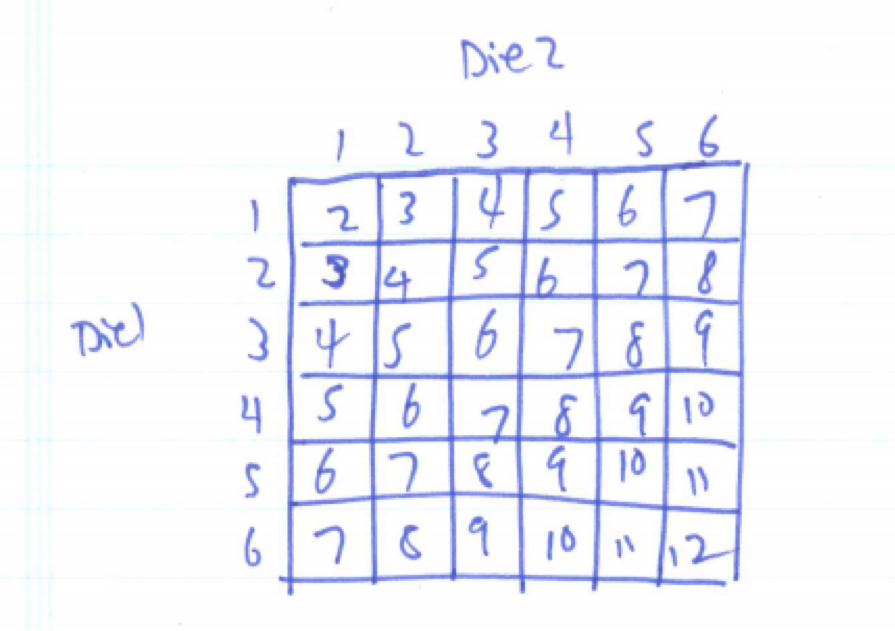
\includegraphics[width=0.3\linewidth]{01-basics-figures/two_dice_sample_space} 

}

\caption{Sample Space for Two Dice}\label{fig:nice-fig-23}
\end{figure}

For example, there is only one combination of dice that yields a sum of
2 (that is 1+1) and there is only one combination of dice that yields a
sum of 3 (that is 1+2) but a sum of 3 is twice as likely because when we
distinguish the dice we see 1+2 and 2+1 as distinct options and we get
\(P(sum=2)=1/36\) while \(P(sum=3)=2/36\).

Let's try another one: which is more likely, a sum of 6 or a sum of 7?
From the sample space we see five ways to obtain a 6 and six ways to
obtain a 7 indicating a sum of 7 is more likely. Stated as
probabilities, \(P(sum=6)=5/36\) and \(P(sum=7)=6/36\).

\subsection{Practice}\label{practice}

Which is more likely when tossing two dice, a sum of 3 or a sum of 11?
Explain.

Simply by counting successes in the sample space we find the probability
of compound events.

Let's define a few events for this experiment of tossing two dice and
find the probabilities of related compound events.

E: The sum is even. F: The sum is less than or equal to 5.

It is helpful to identify members of the sample space satisfying each
event.

\begin{figure}

{\centering \includegraphics[width=0.3\linewidth]{01-basics-figures/two_dice_sample_space_with_evevents} 

}

\caption{Sample Space for Two Dice with Events E and F}\label{fig:nice-fig-24}
\end{figure}

We see \(P(E)=18/36=1/2=0.5\) and also note
\(P(not \ E)=18/36=1/2=0.5\). From the sample space, \(P(F)=10/36\) and
\(P(not \ F)=26/36\).

Looking at compound events, recall that \textbf{AND} refers to the
overlap where both events are true so \(P(E \ and \ F)=4/36\).

We think of \textbf{OR} as an inclusive or representing the event one or
the other or both occur. Counting unique elements of the sample space
that are either an even sum or a sum less than or equal to five we see
\(P(E \ or \ F)=24/36\).

Conditional probability is trickier. \(P(E \mid F)\) means the
probability that the sum is even given we know the sum is less than or
equal to five. To handle this, we assume the sum is less than or equal
to five and this narrows down our sample space to 10 possibilities of
which 4 have an even sum yielding \(P(E \mid F)=4/10\).

\begin{figure}

{\centering 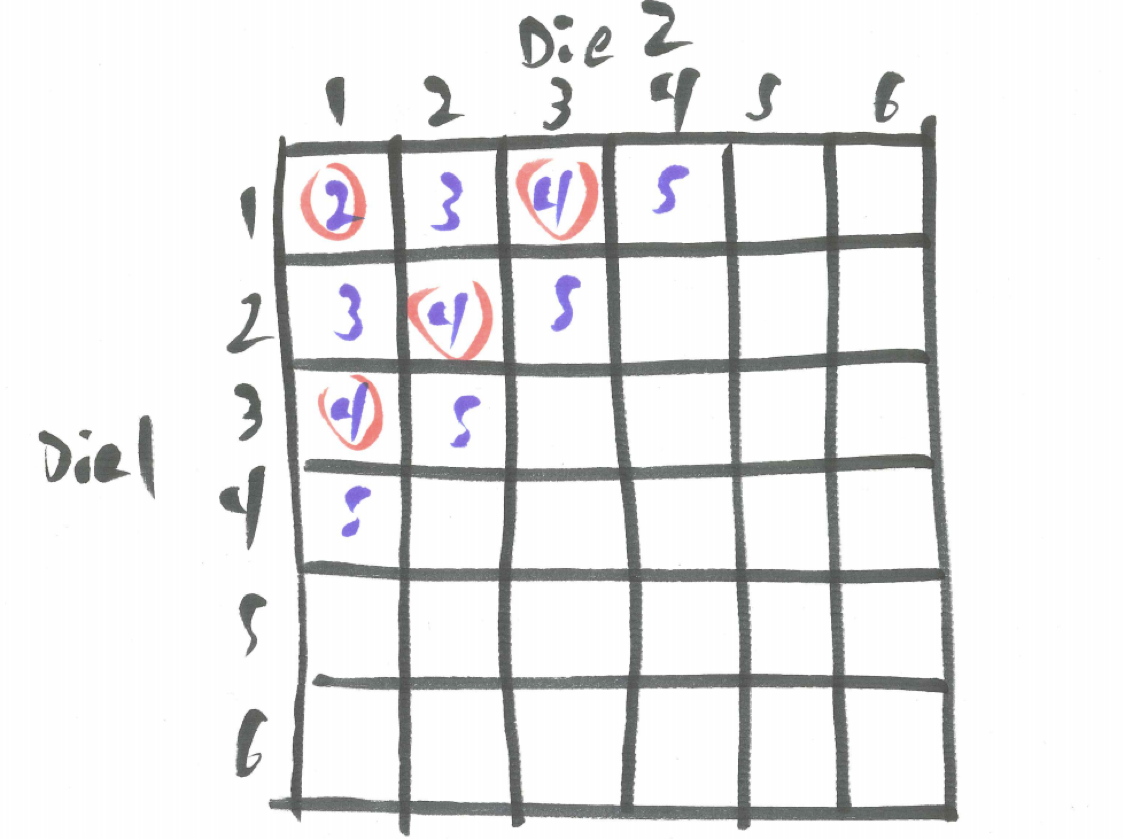
\includegraphics[width=0.3\linewidth]{01-basics-figures/two_dice_sample_space_given_F} 

}

\caption{Sample Space for Two Dice Given F}\label{fig:nice-fig-25}
\end{figure}

It means something quite different to consider \(P(F \mid E)\), the
probability the sum is less than or equal to five given it is even. Out
of the 18 even sums, we find 4 of them are less than or equal to five
yielding \(P(F \mid E)=4/18\).

\begin{figure}

{\centering 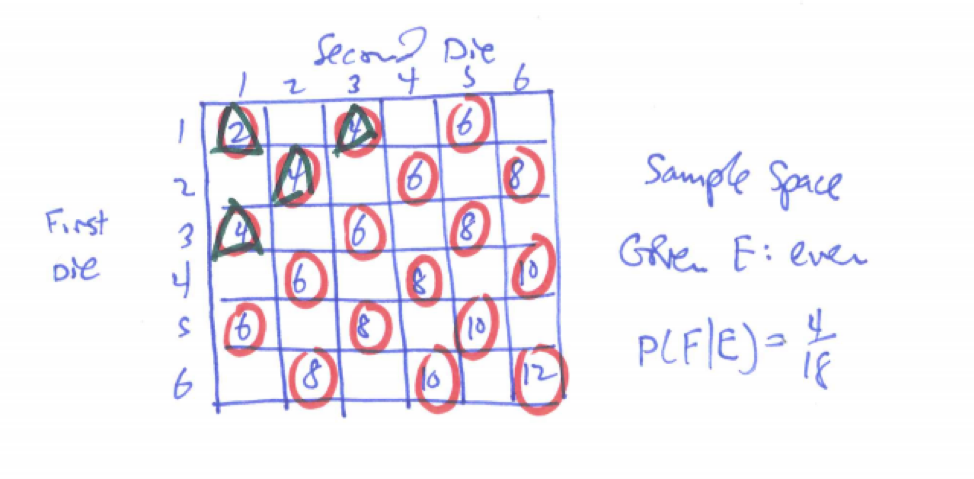
\includegraphics[width=0.3\linewidth]{01-basics-figures/two_dice_sample_space_given_E} 

}

\caption{Sample Space for Two Dice Given E}\label{fig:nice-fig-26}
\end{figure}

It is important to note we found all of the probabilities above by
focusing on the meaning of the events rather than some fancy formula.

\subsection{Practice}\label{practice-1}

For the experiment of tossing two dice with the event D being the sum is
odd and the event T being at least one of the dice is a three find P(D),
P(T), P(not D), P(not T), P(D and T), P(D or T), P(D\textbar{}T), and
P(T\textbar{}D).

\section{Revisiting the Chapter Scenario - Galileo's Dice
Problem}\label{revisiting_chapter_scenario_galileo_dice_problem}

Recall, three dice are tossed. Conventional reasoning indicated a sum of
9 and a sum of 10 should be equally likely as there are six different
dice combinations for each but actual experience indicated the sum of 10
was more likely. To see how Galileo solved this problem we need to
absorb the lesson of pretending we can tell the dice apart.

First of all, since there are 6 equally likely outcomes on each die,
there are \(6 \cdot 6 \cdot 6=216\) total equally likely outcomes in the
sample space.

Let's examine the different combinations of 9 and 10 in the light of
distinguishable dice where order matters.

Sum of Nine

\begin{itemize}
\tightlist
\item
  Combo 1+2+6 - Orderings 1+2+6, 1+6+2, 2+1+6, 2+6+1, 6+1+2, 6+2+1
\item
  Combo 1+3+5 - Orderings 1+3+5, 1+5+3, 3+1+5, 3+5+1, 5+1+3, 5+3+1
\item
  Combo 1+4+4 - Orderings 1+4+4, 4+1+4, 4+4+1
\item
  Combo 2+2+5 - Orderings 2+2+5, 2+5+2, 5+2+2
\item
  Combo 2+3+4 - Orderings 2+3+4, 2+4+3, 3+2+4, 3+4+2, 4+2+3, 4+3+2
\item
  Combo 3+3+3 - Orderings 3+3+3
\end{itemize}

Sum of Ten

\begin{itemize}
\tightlist
\item
  Combo 1+3+6 - Orderings 1+3+6, 1+6+3, 3+1+6, 3+6+1, 6+1+3, 6+3+1
\item
  Combo 1+4+5 - Orderings 1+4+5, 1+5+4, 4+1+5, 4+5+1, 5+1+4, 5+4+1
\item
  Combo 2+2+6 - Orderings 2+2+6, 2+6+2, 6+2+2
\item
  Combo 2+3+5 - Orderings 2+3+5, 2+5+3, 3+2+5, 3+5+2, 5+2+3, 5+3+2
\item
  Combo 2+4+4 - Orderings 2+4+4, 4+2+4, 4+4+2
\item
  Combo 3+3+4 - Orderings 3+3+4, 3+4+3, 4+3+3
\end{itemize}

Tallying the orderings we see there are 25 orderings yielding a sum of 9
and 27 yielding a sum of 10 thus \(P(sum=9)=25/216\) while
\(P(sum=10)=27/216\) and this confirms the real-world experience that a
sum of 10 is actually more likely than a sum of 9.

A simulation might confirm this.

\begin{Shaded}
\begin{Highlighting}[]
\NormalTok{die1 <-}\StringTok{ }\KeywordTok{sample}\NormalTok{(}\DataTypeTok{x=}\DecValTok{1}\OperatorTok{:}\DecValTok{6}\NormalTok{, }\DataTypeTok{size=}\DecValTok{10000}\NormalTok{, }\DataTypeTok{replace =} \OtherTok{TRUE}\NormalTok{)}
\NormalTok{die2 <-}\StringTok{ }\KeywordTok{sample}\NormalTok{(}\DataTypeTok{x=}\DecValTok{1}\OperatorTok{:}\DecValTok{6}\NormalTok{, }\DataTypeTok{size=}\DecValTok{10000}\NormalTok{, }\DataTypeTok{replace =} \OtherTok{TRUE}\NormalTok{)}
\NormalTok{die3 <-}\StringTok{ }\KeywordTok{sample}\NormalTok{(}\DataTypeTok{x=}\DecValTok{1}\OperatorTok{:}\DecValTok{6}\NormalTok{, }\DataTypeTok{size=}\DecValTok{10000}\NormalTok{, }\DataTypeTok{replace =} \OtherTok{TRUE}\NormalTok{)}
\NormalTok{sum3 <-}\StringTok{ }\NormalTok{die1 }\OperatorTok{+}\StringTok{ }\NormalTok{die2 }\OperatorTok{+}\StringTok{ }\NormalTok{die3}
\NormalTok{sim_three_dice <-}\StringTok{ }\KeywordTok{data.frame}\NormalTok{(die1, die2, die3, sum3)}
\NormalTok{knitr}\OperatorTok{::}\KeywordTok{kable}\NormalTok{(}
  \KeywordTok{table}\NormalTok{(sum3), }\DataTypeTok{caption =} \StringTok{'Tossing Three Dice Simulation'}\NormalTok{,}
  \DataTypeTok{booktabs =} \OtherTok{TRUE}
\NormalTok{)}
\end{Highlighting}
\end{Shaded}

\begin{table}

\caption{\label{tab:nice-tab-27}Tossing Three Dice Simulation}
\centering
\begin{tabular}[t]{lr}
\toprule
sum3 & Freq\\
\midrule
3 & 42\\
4 & 131\\
5 & 291\\
6 & 469\\
7 & 700\\
\addlinespace
8 & 992\\
9 & 1138\\
10 & 1229\\
11 & 1255\\
12 & 1156\\
\addlinespace
13 & 1018\\
14 & 654\\
15 & 471\\
16 & 275\\
17 & 133\\
18 & 46\\
\bottomrule
\end{tabular}
\end{table}

\begin{Shaded}
\begin{Highlighting}[]
\KeywordTok{ggplot}\NormalTok{(}\DataTypeTok{data=}\NormalTok{sim_three_dice, }\KeywordTok{aes}\NormalTok{(}\DataTypeTok{x=}\NormalTok{sum3)) }\OperatorTok{+}\StringTok{ }\KeywordTok{geom_histogram}\NormalTok{(}\KeywordTok{aes}\NormalTok{(}\DataTypeTok{y=}\NormalTok{..density..), }\DataTypeTok{binwidth =} \DecValTok{1}\NormalTok{)}
\end{Highlighting}
\end{Shaded}

\begin{figure}

{\centering \includegraphics[width=0.8\linewidth]{probriskreward-bookdown_files/figure-latex/nice-fig-28-1} 

}

\caption{Histogram for Tossing Three Dice}\label{fig:nice-fig-28}
\end{figure}

\chapter{Tree Diagrams}\label{trees}

\section{Introduction}\label{introduction}

In this chapter, tree diagrams are introduced as important tools to
analyze probability questions.

\section{Chapter Scenario - Flipping Two Coins}\label{chapter_scenario}

Imagine a simple situation where two coins are tossed and the number of
heads is observed and the outcome has some relevance for you depending
on whether the result yields 0, 1, or 2 heads. Do you think each of
these outcomes is equally likely? What do you think is the probability
of each of these outcomes?

We use this coin-flipping scenario as a primary example not because we
have inherent interest flipping coins but because this scenario is an
effective model for many real-world situations such as gene inheritance.

\section{Terminology Review}\label{terminology_review}

We have described \textbf{probability} as the measure of the likelihood
of an event on a scale of 0 to 1 with 0 meaning certain failure and 1
meaning certain success.

\[Probability = \frac{successes}{total}\]

Consider a coin is flipped and we examine whether it lands on heads or
tails. We say it is a fair coin if heads and tails are equally likely.
In this case, the probability of the coin landing on heads is \(1/2\)
which can also be expressed as \(0.5\) or \(50\%\) meaning that as the
experiment is repeated the proportion of heads ultimately approaches
\(0.50\). Of course, sample vary so in any given number of trials the
result may not be exact.

The probability experiment of flipping a coin twice and counting the
number of heads leads to three possible outcomes - 0 heads, 1 head, or 2
heads but this might not be a useful sample space because these three
outcomes may not be equally likely. To explore this, we could gather
data by performing the experiment many times and recording the outcome
but in this case a simulation might be faster and provide a larger
sample much more quickly. Besides, you may not have a coin in your
pocket.

\section{Simulation}\label{simulation}

Simulation is often a helpful tool to explore probability questions like
the question above regarding whether getting 0, 1, or 2 heads when
flipping two coins are all equally likely. The code below simulates
10,000 trials of two coin flips keeping track of the number of heads,
number of tails, and proportion of heads for each trial.

\begin{Shaded}
\begin{Highlighting}[]
\NormalTok{sim_}\DecValTok{2}\NormalTok{ <-}\StringTok{ }\KeywordTok{do}\NormalTok{(}\DecValTok{10000}\NormalTok{)}\OperatorTok{*}\KeywordTok{rflip}\NormalTok{(}\DataTypeTok{n=}\DecValTok{2}\NormalTok{, }\DataTypeTok{prob=}\DecValTok{1}\OperatorTok{/}\DecValTok{2}\NormalTok{)}
\NormalTok{knitr}\OperatorTok{::}\KeywordTok{kable}\NormalTok{(}
  \KeywordTok{head}\NormalTok{(sim_}\DecValTok{2}\NormalTok{), }\DataTypeTok{caption =} \StringTok{'Table 1: Two Coin Simulation'}\NormalTok{,}
  \DataTypeTok{booktabs =} \OtherTok{TRUE}
\NormalTok{)}
\end{Highlighting}
\end{Shaded}

\begin{table}

\caption{\label{tab:nice-tab-31}Table 1: Two Coin Simulation}
\centering
\begin{tabular}[t]{rrrr}
\toprule
n & heads & tails & prop\\
\midrule
2 & 0 & 2 & 0.0\\
2 & 0 & 2 & 0.0\\
2 & 1 & 1 & 0.5\\
2 & 2 & 0 & 1.0\\
2 & 1 & 1 & 0.5\\
2 & 2 & 0 & 1.0\\
\bottomrule
\end{tabular}
\end{table}

The result is visualized in a histogram of the \texttt{heads} variable
showing the frequency of obtaining 0, 1, and 2 heads.

\begin{Shaded}
\begin{Highlighting}[]
\KeywordTok{ggplot}\NormalTok{(}\DataTypeTok{data=}\NormalTok{sim_}\DecValTok{2}\NormalTok{, }\KeywordTok{aes}\NormalTok{(}\DataTypeTok{x=}\NormalTok{heads)) }\OperatorTok{+}\StringTok{ }\KeywordTok{geom_histogram}\NormalTok{(}\KeywordTok{aes}\NormalTok{(}\DataTypeTok{y=}\NormalTok{..density..), }\DataTypeTok{binwidth =} \DecValTok{1}\NormalTok{)}
\end{Highlighting}
\end{Shaded}

\begin{figure}

{\centering \includegraphics[width=0.8\linewidth]{probriskreward-bookdown_files/figure-latex/nice-fig-32-1} 

}

\caption{Histogram for Number of Heads When Flipping Two Coins}\label{fig:nice-fig-32}
\end{figure}

Examining the histogram we see that obtaining one head is more likely
than the other two options and, thus, getting 0, 1, and 2 heads when
flipping two coins are not equally likely outcomes. Prompted by the
results of the simulation, we want to know why getting one head is more
likely and tree diagrams will help us.

\section{Tree Diagrams}\label{tree_diagrams}

The outcomes of a probability experiment can be catalogued with a tree
diagram where at each node the different branches represent the
different possible outcomes at each stage of the process.

Consider the tree diagram for flipping a single coin where we label each
node as either H for Heads or T for tails and label the probability
along each branch.

\begin{figure}

{\centering 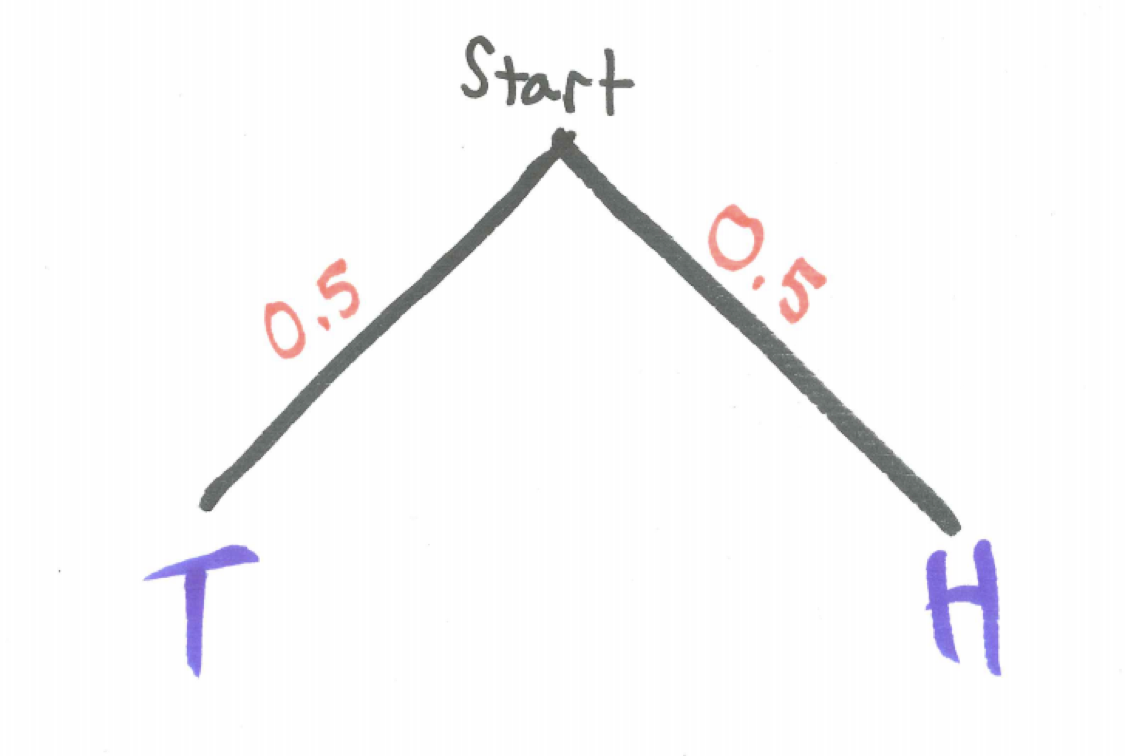
\includegraphics[width=0.3\linewidth]{01-basics-figures/tree_one_coin} 

}

\caption{Tree Diagram for One Coin}\label{fig:nice-fig-33}
\end{figure}

Including the possible outcomes for a second coin results in a tree
diagram with four branches.

\begin{figure}

{\centering 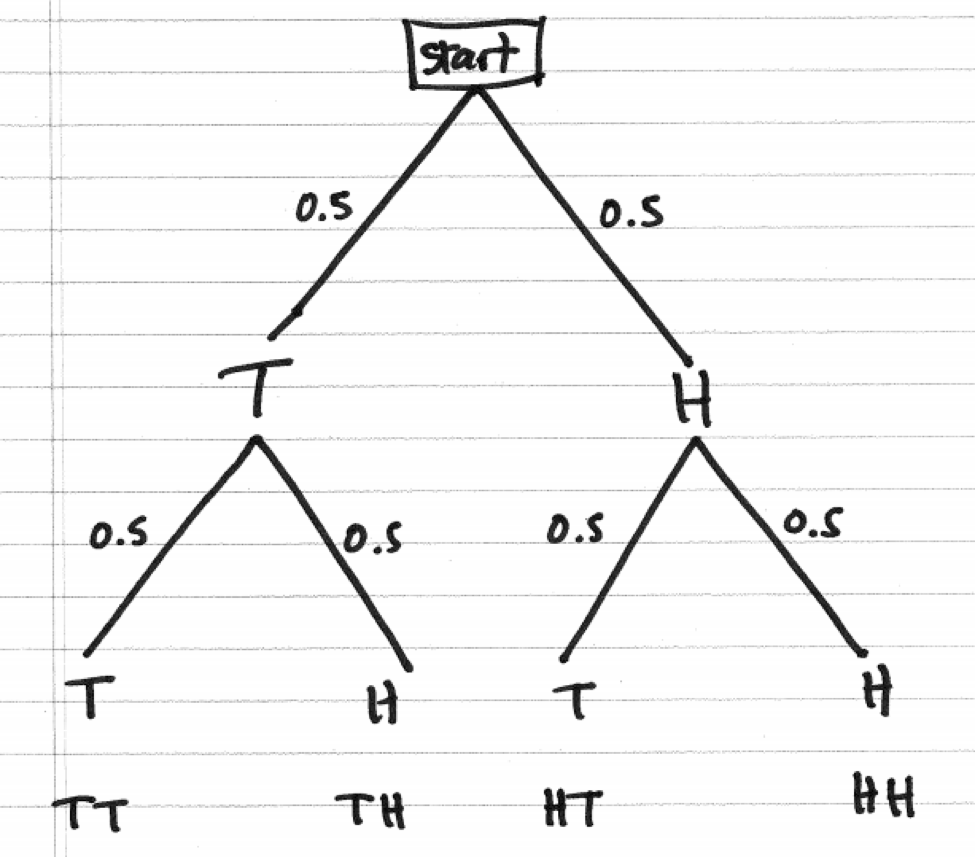
\includegraphics[width=0.6\linewidth]{01-basics-figures/tree_two_coins} 

}

\caption{Tree Diagram for Two Coins}\label{fig:nice-fig-34}
\end{figure}

Each path from the top of the tree to the bottom represents one possible
outcome when tossing two coins. In this experiment, there is a 50/50
chance of getting heads or tails thus all four paths are equally likely
each occurring with probability \(0.5 \times 0.5 = 0.25\). If we think
of the probability associated with each branch as the proportion of the
time we travel down that branch then multiplying these probabilities
makes perfect sense to determine the probability of traveling down
sequential branches.

We can now understand why getting one head is more likely as there are
two paths, HT and TH, compared to only one path generating zero heads,
TT, and only one path generating two heads, HH, resulting in the
following probabilities:

\[P(0\ heads) = P(TT) = (0.5)(0.5) = 0.25\]
\[\small P(1\ head) = P(TH\ or\ HT) = P(TH) + P(HT) = (0.5)(0.5) + (0.5)(0.5) = 0.25 + 0.25 = 0.5\]

\[P(2\ heads) = P(HH) = (0.5)(0.5) = 0.25\]

\section{An Example with Rats}\label{an_example_with_rats}

Now consider the experiment of choosing three rats at random from a
large population of rats that is 40\% male and 60\% female. Just as we
did for coins, we can draw a tree diagram with branches representing the
sex of the first, second, and third rat chosen and label the associated
probabilities on each branch. Selecting the rats and identifying gender
would be equivalent to having a coin that lands on one side 40\% of the
time and on the other 60\% of the time. In the tree diagram below, we
have added subscripts to identify whether we are referring to the first,
second, or third rat selected.

\begin{figure}

{\centering 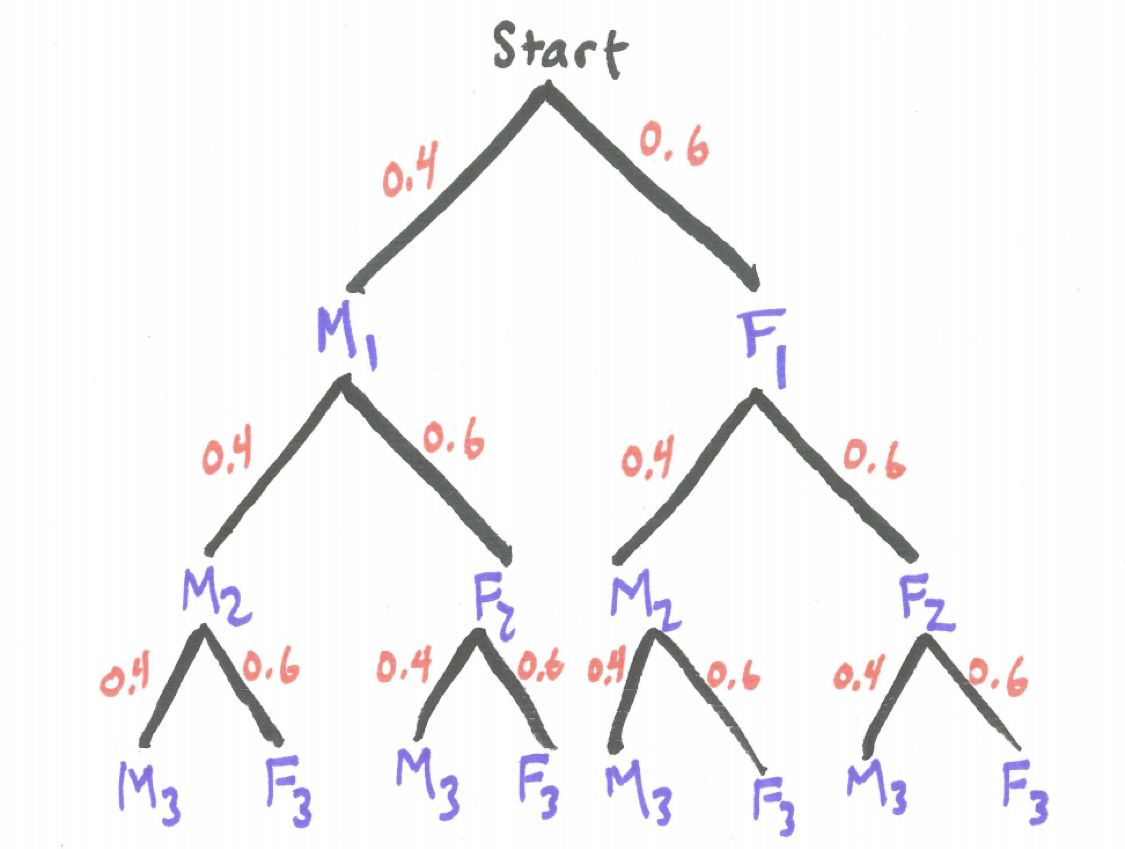
\includegraphics[width=0.6\linewidth]{01-basics-figures/tree_rat_sex} 

}

\caption{Tree Diagram for Three Rats}\label{fig:nice-fig-35}
\end{figure}

What is the probability of selecting 0 female rats? Note that because
the population is large at each stage of the process the probability of
selecting a female rat remains for all practical purposes 0.60.

\[P(0\ female\ rats) = P(M_{1}\ and\ M_{2}\ and\ M_{3}) = (0.4) \times (0.4) \times (0.4) = 0.064\]

What is the probability of selecting 1 female rat? There are actually
three distinct paths through the tree where 1 female rat and 2 male rats
are selected and each one has the probability \((0.6) \times (0.4)^2\)
thus the probability is

\[P(1\ female\ rat) = 3 \times (0.6) (0.4)^2 = 0.288\]

\subsection{Practice Exercise}\label{practice-exercise-5}

For the probability experiment described above, choosing three rats at
random from a large population of rats that is 40\% male and 60\%
female, what is the probability of getting 2 female rats? 3 female rats?

\section{The Urn Model}\label{the_urn_model}

When confronted with a question of personal importance to you where
probabilistic concerns are relevant to getting an accurate answer, the
ability to develop a model that captures important probability details
is a key problem-solving tool. By \textbf{model} we mean a systematic
description that shares all of the important characterics of the
problem, be it a physical, visual, mathematical, or computational
representation (\url{http://www.dictionary.com/browse/model}).

For probability experiments two useful models are the coin-flipping
model and the urn model. We have already looked briefly at a
coin-flipping experiment. We will see throughout our probabilistic
treatment of genetics that we will often use coin-flipping as a mental
model to think about questions of genetic risk and reward. The urn model
is another important way to think about probability questions.

Consider an urn with some beads in it. Imagine the urn has 20 beads 12
of which are black and 8 white and we are to draw out three of these
beads at random and we want to find the probability of ending up with 0,
1, 2, or 3 black beads.

\begin{figure}

{\centering 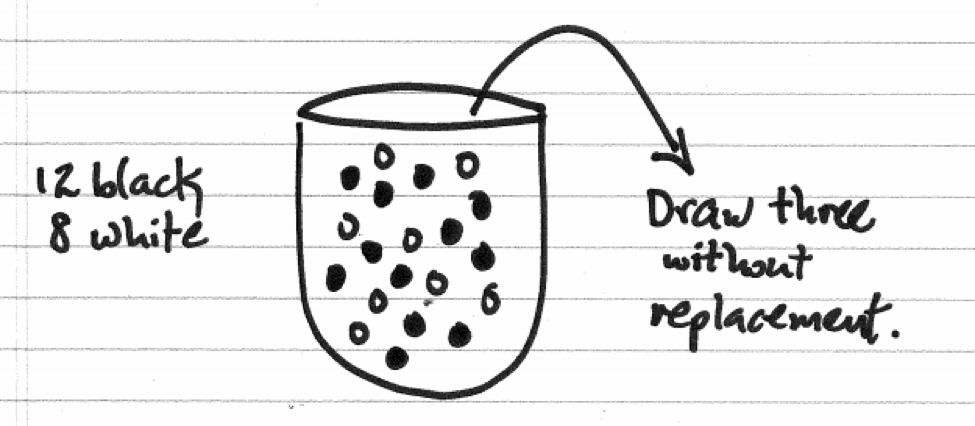
\includegraphics[width=0.6\linewidth]{01-basics-figures/urn1_picture} 

}

\caption{The Urn Model}\label{fig:nice-fig-36}
\end{figure}

First, we need to be clear up one question: is the drawing out of beads
to be done with replacement or without replacement? By \textbf{with
replacement} we mean that after each draw of one bead, it is replaced,
the beads thoroughly mixed, before another bead is selected at random.
By \textbf{without replacement} we mean that after one bead is removed,
it is not replaced before the next bead is selected. Note, if we are
selecting three beads at once this could be viewed as equivalent to
selecting the beads one at a time without replacement.

\begin{figure}

{\centering 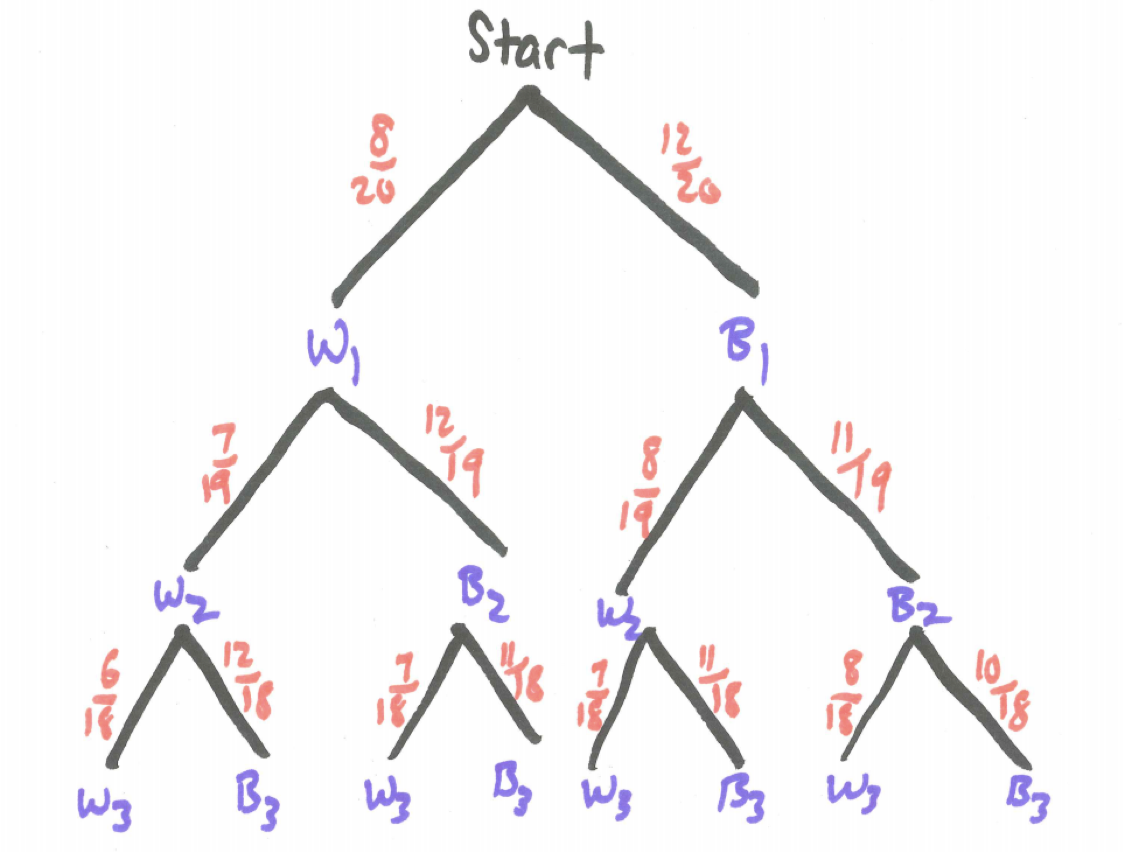
\includegraphics[width=0.6\linewidth]{01-basics-figures/tree_urn1} 

}

\caption{Tree Diagram for Three Beads}\label{fig:nice-fig-37}
\end{figure}

For this experiment with three beads drawn at random without replacement
from an urn containing 12 black and 8 white beads, what is the
probability of ending up with 0, 1, 2, or 3 black beads, respectively?

First, let's tackle the probability of getting 0 black beads. From
examining the tree we see

\[P(0\ blacks) = P(W_{1}\ and\ W_{2}\ and\ W_{3}) = \frac{8}{20} \times \frac{7}{19} \times \frac{6}{18}\]

Finding the probability of one black is more work. As we examine the
tree we see there are three distinct paths resulting in one black. Check
out their separate probabilities here.

\[P(B_{1}\ and\ W_{2}\ and\ W_{3}) = \frac{12}{20} \times \frac{8}{19} \times \frac{7}{18} = 0.098\]

\[P(W_{1}\ and\ B_{2}\ and\ W_{3}) = \frac{8}{20} \times \frac{12}{19} \times \frac{7}{18} = 0.098\]

\[P(W_{1}\ and\ W_{2}\ and\ B_{3}) = \frac{8}{20} \times \frac{7}{19} \times \frac{12}{18} = 0.098\]

In spite of the numerators being in different orders, we notice that
these three separate probabilities are numerically equal. Thus, for the
final probability we see

\[P(1\ black) = 3 \times \frac{12}{20} \times \frac{8}{19} \times \frac{7}{18} = 0.295\]

\subsection{Practice Exercise}\label{practice-exercise-6}

For the urn described above containing 12 black and 8 white beads with
three beads drawn at random without replacement, what is the probability
of obtaining two black beads? What is the probability of obtaining three
black beads?

\section{Exercises}\label{exercises}

\subsection{Exercise - Three Coins in the
Fountain}\label{exercise---three-coins-in-the-fountain}

A penny, a nickel, and a dime are all flipped at the same time. Draw an
appropriate tree diagram with associated probabilities labeled on each
branch and find the probabilities of the following events: obtaining no
heads, obtaining exactly one head, exactly two heads, and exactly three
heads.

\subsection{Exercise - More Coins}\label{exercise---more-coins}

Draw a tree diagram for the probability experiment of flipping four
coins. Label each node as either H for Heads or T for tails and label
the probability along each branch. Find the probability of obtaining no
heads and the probability of obtaining at least one head and describe
the relationship between these two probabilities.

\subsection{Exercise - Class
Committee}\label{exercise---class-committee}

Consider the experiment of selecting a committee of three individuals
from a class of 20 of which 8 are male and 12 are female. Draw a tree
diagram with associated probabilities for the gender of the first,
second, and third person chosen for the committee and find the
probabilities the committee consists of 0 females, 1 female, 2 females,
and 3 females, respectively.

\chapter{Interlude - In an Attempt to Kill the Student, the Authors
Solve the Same Simple Problem Four Ways (One Bad and Three
Good)}\label{kill_the_student}

By dissecting an easy problem we can gain insight into multiple
problem-solving strategies that can be useful in other problems. Or we
can kill motivation altogether. We will see.

In this interlude, we see one example worked multiple ways. The specific
problem-solving tools will be expounded upon in subsequent chapters.

\section{A Problem from the Game of Risk}\label{risk_problem}

In the game of Risk competitors resolve attacks by rolling dice. Suppose
that you are rolling two dice and you are interested in whether or not
we obtain a six. We consider the following compound events.

While there are six sides to each die, because we are primarily
interested in whether or not we obtain a six, we will use the tree
diagram below where event \textbf{S} represents getting a six and event
\textbf{N} represents getting a non-six, ie., 1, 2, 3, 4, or 5.

\begin{figure}

{\centering 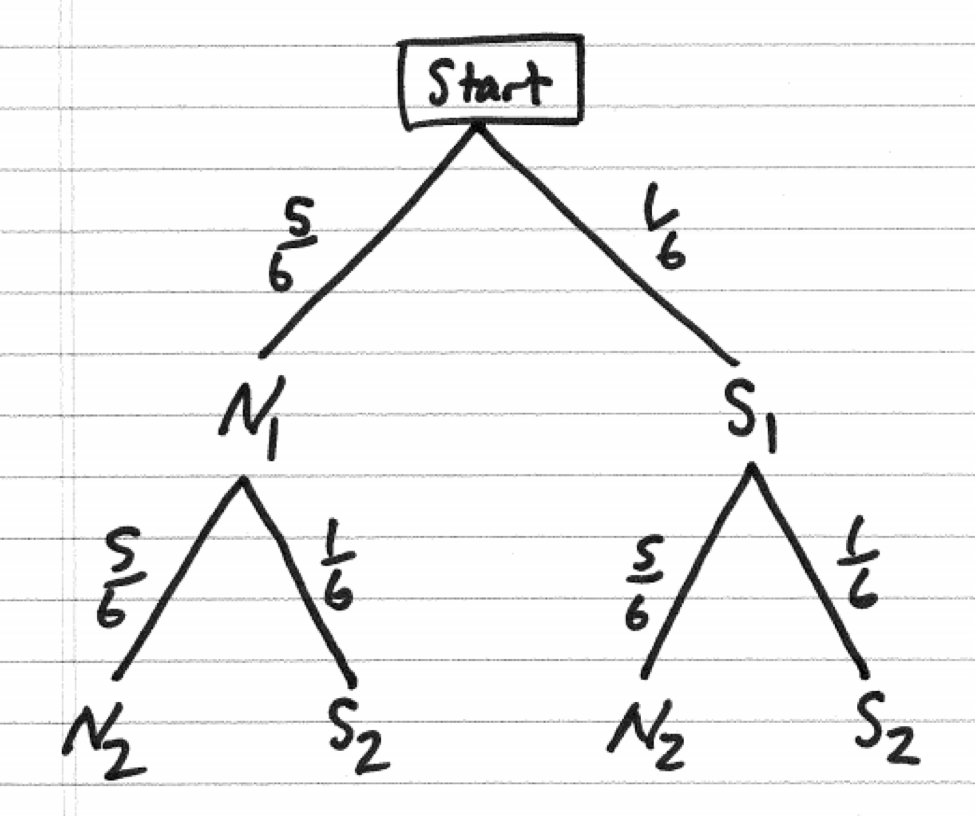
\includegraphics[width=0.6\linewidth]{01-basics-figures/tree_two_dice_sixes} 

}

\caption{Tree Diagram for Sixes on Two Dice}\label{fig:nice-fig-41}
\end{figure}

Even if we are tossing identical dice simultaneously it is helpful to
conceptualize the experiment as if we are tossing the dice sequentially.
We have added subscripts to identify whether we are referring to the
first die tossed or the second die tossed.

What is the probability of obtaining a six on both dice? Because the two
events of getting a six on the first die and getting a six on the second
die are \textbf{independent}, we can use \textbf{The Multiplication Rule
for Independent Events} which says for any two independent events \(E\)
and \(F\), \(P(E\ and\ F) = P(E) \times P(F)\).

\[P(two\ sixes) = P(S_{1}\ and\ S_{2}) = P(S_{1}) \times P(S_{2}) =  \frac{1}{6} \times \frac{1}{6}\]

What is the probability of obtaining a six on at least one of the two
dice? We examine this problem from four points of view - the wrong point
of view, the addition rule, the partition technique, and the complement
principle.

\subsubsection{The Wrong Way}\label{the-wrong-way}

Here is a faulty answer:

\[P(at\ least\ one\ six) = P(S_{1}\ or\ S_{2}) = P(S_{1})+ P(S_{2}) = \frac{1}{6} + \frac{1}{6} = \frac{2}{6} = \frac{1}{3}\ \ WRONG!\]

Can you spot the problem? The issue is that one branch with a six on
both dice, the overlap where both events \(S_{1}\) and \(S_{2}\) occur,
was counted twice.

\subsubsection{The Addition Rule}\label{the-addition-rule}

Here is a correct version using what is called \textbf{The Addition
Rule} where the overlap, since it was counted twice, is subtracted:

\[P(at\ least\ one\ six) = P(S_{1}\ or\ S_{2}) = P(S_{1})+ P(S_{2}) - P(S_{1}\ AND\ S_{2}) =\\ \frac{1}{6} + \frac{1}{6} - \frac{1}{6} \times \frac{1}{6}  = \frac{11}{36}\]

\subsubsection{The Partition Approach}\label{the-partition-approach}

An alternative approach is to \textbf{partition} the event into mutually
exclusive parts. We might informally describe this approach as
\emph{divide and conquer}. In this case, there are three distinct
branches that satisfy at least one six occurring:

\[P(at\ least\ one\ six) = P(S_{1}\ and\ N_{2}) + P(N_{1}\ and\ S_{2}) + P(S_{1}\ and\ S_{2}) = \\  \frac{1}{6} \times \frac{5}{6} + \frac{5}{6} \times \frac{1}{6} + \frac{1}{6} \times \frac{1}{6} = \frac{11}{36}\]

\subsubsection{The Complement Principle}\label{the-complement-principle}

A third correct approach uses \textbf{The Complement Principle} which
observes that for any event \(E\), \(P(E) = 1 - P(not\ E)\). In this
situation, we note \(P(at\ least\ one) = 1 - P(none)\). Sometimes it is
less work to find the complement of an event and subtract from one.

\[P(at\ least\ one\ six) = 1 - P(no\ sixes) = 1 - P(N_{1}\ and\ N_{2}) = \\  1 - \frac{5}{6} \times \frac{5}{6} = \frac{11}{36}\]

To summarize what we have learned about problem-solving here, there is
more than one way to solve a probability problem (and some ways are
wrong!). But several good strategies to use are the addition rule being
careful not to double-count, divide and conquer by partitioning the
event into mutually exclusive pieces, or use the complement principle to
solve the opposite problem and subtract this from one.

\chapter{Working with OR Statements}\label{working_with_or_statements}

\section{Introduction}\label{introduction}

Most of the interesting probability questions involve combinations of
simple events. In this section we examine the probabilities of at least
one of two events occurring (\textbf{or}), and describe the key Addition
Principle. Venn diagrams are introduced as useful tools for visualizing
relationships between overlapping events.

\section{Chapter Scenario - Paying
Taxes}\label{chapter_scenario_paying_taxes}

On the Diane Rehm show on Wednesday, September 28, 2016 a discussion of
federal taxes occurred. Here is the link to the show:
\url{https://thedianerehmshow.org/}.

A claim something like the following was made: 55\% of individuals pay
federal income tax, 70\% pay payroll taxes, and 80\% pay at least one of
the two. Can you determine the percentage of individuals that pay
federal income tax but not payroll taxes and the percentage who pay
payroll taxes but not federal income tax?

\section{Class Composition Example}\label{class-composition-example}

Suppose we took a poll of all 25 students in class and asked them to
identify whether or not they were from Utah and whether or not they are
planning to major in a business-related field with the following
results:

\begin{itemize}
\tightlist
\item
  13 are from Utah
\item
  8 plan to major in a business-related field
\item
  5 are from Utah AND plan to major in a business-related field
\end{itemize}

If one student is chosen at random what is the probability they are from
Utah OR plan to major in a business-related field?

Let's let U represent the event of being from Utah and B the event of
planning to major in a buisness-related field.

\subsection{Practice Exercise}\label{practice-exercise-7}

What is wrong with the following approach?

\[P(U \ or \ B) = P(U)+P(B)= 13/25 + 8/25 = 21/25 \ WRONG!!!\]

You may have spotted the mistake that some individuals have been
double-counted. The Addition Principle will take care of this.

\[P(U \ or \ B) = P(U)+P(B)-P(U \ and \ B) = 13/25 + 8/25 - 5/25 = 16/25\]

From the information above we can determine there are 9 individuals that
are not from Utah and not planning on majoring in business-related
field. Venn Diagrams are a helpful way to visualize the relationships
between overlapping events like these.

Two overlapping events may be represented in a Venn diagram with two
overlapping circles. Think of the rectangle containing them as the
entire sample space.

Examine the three Venn diagrams below. The first Venn diagram
illustrates the compound event each region represents. The second Venn
diagram identifies the number of individuals in each region. The third
Venn diagram identifies the proportion of the population in each region,
or, equivalently, the probability of selecting an individual in the
given region if one person was chosen at random.

\begin{figure}

{\centering \includegraphics[width=0.3\linewidth]{01-basics-figures/venn_class_composition} 

}

\caption{Venn Diagram of Class Composition}\label{fig:nice-fig-51}
\end{figure}

\section{Venn Diagrams for Three
Events}\label{venn-diagrams-for-three-events}

A Venn diagram for three overlapping events is represented with three
overlapping circles creating the eight regions all labeled in the
diagram below. By the Fundamental Principle of Counting, to identify a
region there are two choices for each event - out or in - leading to
\(2^{3}=8\) total regions.

\begin{figure}

{\centering 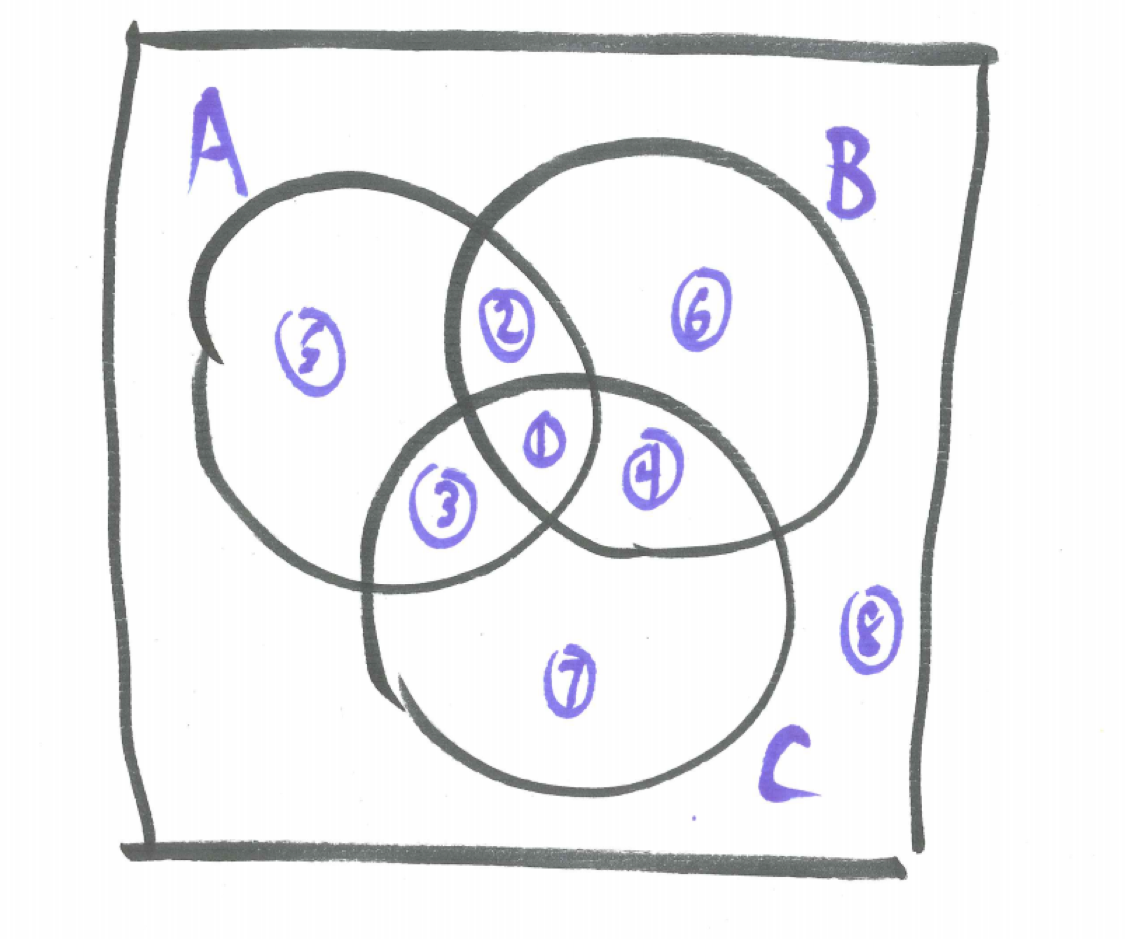
\includegraphics[width=0.3\linewidth]{01-basics-figures/venn_three_events} 

}

\caption{Venn Diagram of Three Events}\label{fig:nice-fig-52}
\end{figure}

\section{Example - Watching Sports}\label{example---watching-sports}

A group of students was asked whether or not they like to watch
basketball, soccer, and/or football. Here are the results of the survey.

\begin{itemize}
\tightlist
\item
  Total number surveyed: 78
\item
  Number choosing basketball: 26
\item
  Number choosing soccer: 30
\item
  Number choosing football: 36
\item
  Number choosing both basketball and soccer: 10
\item
  Number choosing both basketball and football: 12
\item
  Number choosing both soccer and football: 18
\item
  Number choosing basketball and soccer and football: 8
\end{itemize}

We can draw a Venn Diagram by identifying with regions B for basketball,
S for soccer, F for football, and T representing the total number
surveyed. We want to determine how many individuals there are in each of
the eight regions. As in the example with two overlapping events, the
key problem-solving strategy is to start with the overlap.

\section{Revisiting the Chapter Scenario - Paying
Taxes}\label{revisit_chapter_scenario}

Remember in our example, 55\% of individuals pay federal income tax,
70\% pay payroll taxes, and 80\% pay at least one of the two and we wish
to determine the percentage of individuals that pay federal income tax
but not payroll taxes and the percentage who pay payroll taxes but not
federal income tax. A Venn diagram can help with F representing federal
income tax and P payroll taxes.

From the Addition Principle,

\[P(F \ or \ P)=P(F)+P(P)-P(F \ and \ P)\] We know three of these
quantities which may be substituted in.

\[0.80=0.55+0.70-P(F \ and \ P)\]

Solving we find \(P(F \ and \ P)=0.55 + 0.70 - 0.80=0.45\) allowing us
to complete the Venn diagram.

\begin{figure}

{\centering 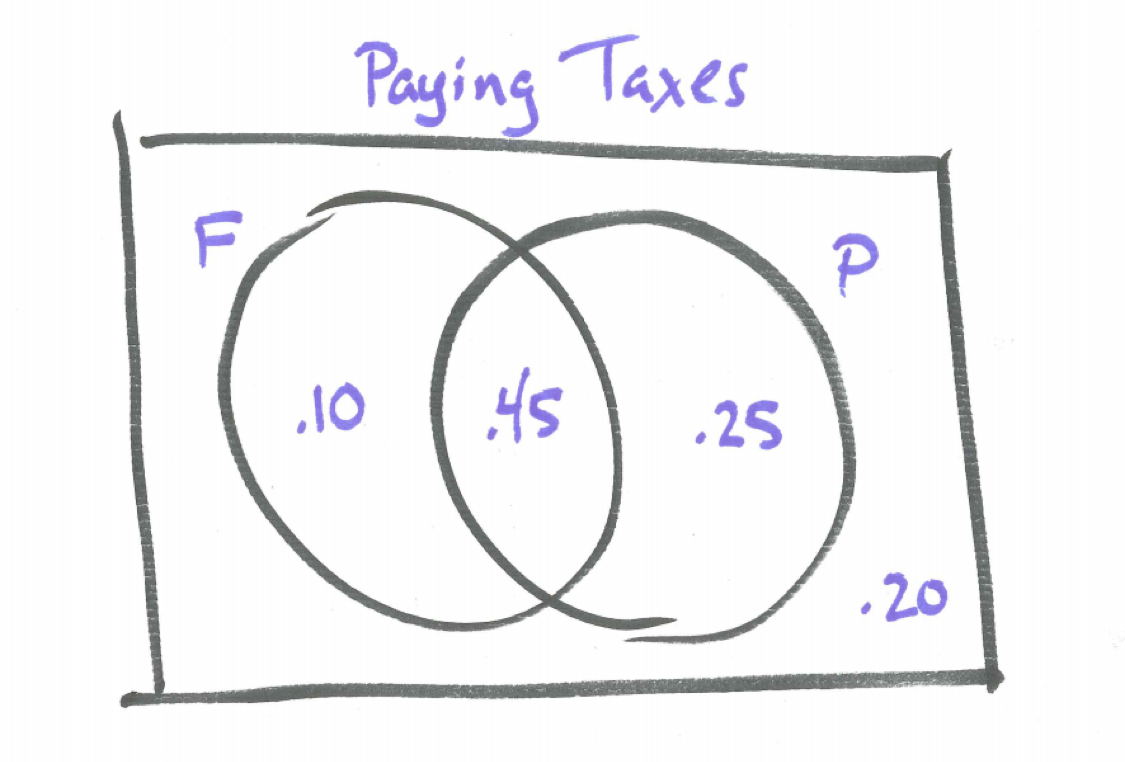
\includegraphics[width=0.3\linewidth]{01-basics-figures/venn_paying_taxes} 

}

\caption{Venn Diagram of Paying Taxes}\label{fig:nice-fig-53}
\end{figure}

\section{Exercises}\label{exercises}

\subsection{Exercise - Venn for Four}\label{exercise---venn-for-four}

Create a Venn diagram template for four events \{A, B, C, D\} and
accurately label each region.

\subsection{Exercise - Class
Schedules}\label{exercise---class-schedules}

Suppose that a group of 100 first year students were given a survey
indicating that 58 of them are registered for a math class and 40 of
them are registered for a foreign language class. Can we safely assume
that 98 of them are registered for either a math class or a foreign
language class? Suppose we are told that 22 of them are registered for
both a math class and a foreign language class, then determine how many
are registered for a math class or a foreign language class.

\subsection{Exercise - Class Survey}\label{exercise---class-survey}

Design and administer a short three-question class survey where each
question is a yes or no answer and draw a Venn diagram of the results
identifying the number of individuals in each of the eight regions.
Questions could relate to almost anything but try to select questions
where you will see different responses.

\chapter{Working with AND and NOT
Statements}\label{working_with_and_and_not_statements}

\section{Introduction}\label{introduction}

Most of the interesting probability questions involve combinations of
simple events. In this section we examine the probabilities of two
events both occurring (\textbf{and}) as well as an event not occurring
(\textbf{not}). In this chapter,we describe the key probability
principles related to \textbf{and}, and \textbf{not} statements, namely,
the Multiplication Principle and Complement Principle, respectively.

\section{Chapter Scenario - The Birthday
Problem}\label{chapter_scenario_birthday_problem}

You may be sitting in a classroom right now. If not, imagine you are.
Suppose there are a total of 20 people in class. What is the chance that
two of you have the same birthday (meaning same day of the year but not
necessarily the same year)? Which is it closer to - a 10\%, 20\%, 30\%,
40\%, or 50\% chance, or possibly even higher chance?

\section{The Chevalier de Mere}\label{the-chevalier-de-mere}

Aaah, the ``Horseman of the Sea,'' that famous gambler who had a horse
and lived by the sea. And who was, by the way, an acquaintance of
Pascal, owner of famous triangle in the year 1654. There were two games
of chance that the Chevalier wanted some advice on and he wrote Pascal
and letter and, viola, the theory of probability was born. OK, it wasn't
that simple but the Chevalier's question did stimulate a deeper
understanding of probability intimating at what we now call the
multiplication rule and the complement rule. Here are the two games
under consideration -

Game One: You could bet on the chance of getting at least one six on
four rolls of a die.

Game Two: For a longer game, you could bet on the chance of getting at
least one double six on 24 rolls of two dice.

\subsection{Practice Exercise}\label{practice-exercise-8}

Estimate the probability of winning Game One and the probability of
winning Game Two. No formal computation necessary at this point. Each of
these games was an even-money game meaning the payoff ratio was 1:1
where you would either win or lose the exact amount bet. The Chevalier
de Mere had a lot of experience and felt that the first game offered a
better chance of winning than the second game but he could find no
theoretical explanation as to why. In his mind, with the prevailing math
at the time, the two games seemed comparable. If I am given 4 tries to
get something that happens on average every 6 times then being given 24
tries at something that happens on average every 36 times should be
comparable. But in reality it was not. In short, his mathematical
reasoning was letting him down.

We can use simulation to recreate the Chevalier's experience. The code
below simulates 10,000 trials of Game One and documents the number of
wins and losses.

\begin{Shaded}
\begin{Highlighting}[]
\NormalTok{die_tosses <-}\StringTok{ }\KeywordTok{matrix}\NormalTok{(}\KeywordTok{sample}\NormalTok{(}\DecValTok{1}\OperatorTok{:}\DecValTok{6}\NormalTok{, }\DecValTok{4}\OperatorTok{*}\DecValTok{10000}\NormalTok{, }\DataTypeTok{replace=}\OtherTok{TRUE}\NormalTok{), }\DataTypeTok{ncol=}\DecValTok{4}\NormalTok{) }\CommentTok{#generate die tosses}
\NormalTok{sixes_logic <-}\StringTok{ }\NormalTok{die_tosses}\OperatorTok{==}\DecValTok{6} \CommentTok{#identify where there are sixes (TRUE=1, FALSE=0)}
\NormalTok{number_of_sixes <-}\StringTok{ }\KeywordTok{apply}\NormalTok{(sixes_logic, }\DecValTok{1}\NormalTok{, sum) }\CommentTok{#Tabulate the number of sixes in each game}
\NormalTok{game_one_winners <-}\StringTok{ }\NormalTok{number_of_sixes }\OperatorTok{>}\StringTok{ }\DecValTok{0} \CommentTok{#Identify the winners - those with at least one six}

 \CommentTok{#Calculate the proportion of game one winners}
\NormalTok{knitr}\OperatorTok{::}\KeywordTok{kable}\NormalTok{(}
  \KeywordTok{prop.table}\NormalTok{(}\KeywordTok{table}\NormalTok{(game_one_winners)), }\DataTypeTok{caption =} \StringTok{'Game One Simulation'}\NormalTok{,}
  \DataTypeTok{booktabs =} \OtherTok{TRUE}
\NormalTok{)}
\end{Highlighting}
\end{Shaded}

\begin{table}

\caption{\label{tab:nice-tab-61}Game One Simulation}
\centering
\begin{tabular}[t]{lr}
\toprule
game\_one\_winners & Freq\\
\midrule
FALSE & 0.4861\\
TRUE & 0.5139\\
\bottomrule
\end{tabular}
\end{table}

The simulated Chevalier in this simulation would notice winning
\(51.39\%\) of the time. Let's simulate 10,000 trials of Game Two for
comparison sake.

\begin{Shaded}
\begin{Highlighting}[]
\NormalTok{two_Die_tosses <-}\StringTok{ }\KeywordTok{matrix}\NormalTok{(}\KeywordTok{sample}\NormalTok{(}\DecValTok{1}\OperatorTok{:}\DecValTok{6}\NormalTok{, }\DecValTok{24}\OperatorTok{*}\DecValTok{10000}\NormalTok{, }\DataTypeTok{replace=}\OtherTok{TRUE}\NormalTok{) }\OperatorTok{+}\StringTok{ }
\StringTok{    }\KeywordTok{sample}\NormalTok{(}\DecValTok{1}\OperatorTok{:}\DecValTok{6}\NormalTok{, }\DecValTok{24}\OperatorTok{*}\DecValTok{10000}\NormalTok{, }\DataTypeTok{replace=}\OtherTok{TRUE}\NormalTok{), }\DataTypeTok{ncol=}\DecValTok{24}\NormalTok{) }\CommentTok{#generate 10000 trials of 24 two dice rolls}
\NormalTok{double_sixes_logic <-}\StringTok{ }\NormalTok{two_Die_tosses}\OperatorTok{==}\DecValTok{12} \CommentTok{#identify double sixes (TRUE=1, FALSE=0)}
\CommentTok{#head(double_sixes_logic, n=10) }
\NormalTok{number_of_double_sixes <-}\StringTok{ }\KeywordTok{apply}\NormalTok{(double_sixes_logic, }\DecValTok{1}\NormalTok{, sum) }\CommentTok{#tabulate number of double sixes in each game}
\NormalTok{game_two_winners <-}\StringTok{ }\NormalTok{number_of_double_sixes }\OperatorTok{>}\StringTok{ }\DecValTok{0} \CommentTok{#identify winners - those with at least one double six}

\CommentTok{#Calculate the proportion of game two winners}
\NormalTok{knitr}\OperatorTok{::}\KeywordTok{kable}\NormalTok{(}
  \KeywordTok{prop.table}\NormalTok{(}\KeywordTok{table}\NormalTok{(game_two_winners)), }\DataTypeTok{caption =} \StringTok{'Game Two Simulation'}\NormalTok{,}
  \DataTypeTok{booktabs =} \OtherTok{TRUE}
\NormalTok{)}
\end{Highlighting}
\end{Shaded}

\begin{table}

\caption{\label{tab:nice-tab-62}Game Two Simulation}
\centering
\begin{tabular}[t]{lr}
\toprule
game\_two\_winners & Freq\\
\midrule
FALSE & 0.5096\\
TRUE & 0.4904\\
\bottomrule
\end{tabular}
\end{table}

This time, our simulated Chevalier sees he is winning only \(49.04\%\)
of the time. Hence the rub. Why is Game One better than Game Two?

Enter Pascal, stage right. Here we let you do a little play-acting and
audition for the role of Pascal by analyzing the games and determining
the chances of winning each. To do this, let's explore what we now call
the multiplication rule and the complement rule.

The Multiplication Rule shows us that to obtain the probability of two
potentially consecutive events we multiply related probabilities:

\subsection{Theorem: The Multiplication
Principle}\label{theorem-the-multiplication-principle}

\[For \ all \ events \ A \ and \ B, \ P(A \ and \ B)= P(A) \cdot P(B \mid A).\]

To understand the multiplication principle, examine the tree diagram
below where branches are labeled with the events and the corresponding
probabilities. We see that traveling the \textbf{A and B} branch happens
with probability \(P(A) \cdot P(B \mid A)\).

In the special case that events A and B are independent we note that
\(P(B \mid A) = P(B)\) resulting in the simplified tree diagram below.

This leads to a special case of the multiplication principle.

\subsection{Theorem: Special Case of the Multiplication
Principle}\label{theorem-special-case-of-the-multiplication-principle}

\[If \ the \ events \ A \ and \ B \ are \ independent \ then \ P(A \ and \ B) = P(A) \cdot P(B).\]

The Complement Rule confirms that the probability of an event occurring
is one minus the probability the event does not occur:

\subsection{Theorem: Complement
Principle}\label{theorem-complement-principle}

\[For \ all \ events \ A, \ P(A)= 1-P(not \ A)\]

Remember this can also be written as \(P(A) + P(not \ A) = 1\).

Tackling the Chevalier's problem one die at a time, consider the
experiment of tossing just one die. Suppose we are interested in the
event S of getting a six.

\[P(getting \ a \ six) = P(S) = 1/6\]

This is equivalent to the following version using the complement
principle:

\[P(getting \ a \ six) = 1 – P(not \ getting \ a \ six) = 1 - P(not \ S) = 1 – 5/6 = 1/6\]

Now consider the experiment of tossing two dice. Let \(S_{1}\) represent
getting a six on the first die and \(S_{2}\) getting a six on the second
die. Note that whatever happens on the first die is independent of what
happens on the second die. To find the probability of getting double
sixes we can utilize the multiplication rule.

\[P(two \ sixes)= P(S_{1} \ and \ S_{2})=P(S_{1}) \cdot (S_{2})=  1/6 \cdot 1/6=1/36\]

There is a note of caution here; remember this technique only works with
independent events like dice rolls and would not work for dependent
event like drawing from an urn without replacement.

Similarly, we could now use independence and the Multiplication Rule to
help us understand the event of not getting a six.

\[P(no \ sixes)= P(S_{1}^{c} \ and \ S_{2}^{c}) = P(S_{1}^{c}) \cdot P(S_{2}^{c}) =5/6 \cdot 5/6=25/36\]

We often use the complement rule when finding the probability of at
least one occurrence of an event in multiple trials. To say ``at least
one success'' and to say ``no successes'' are complements of each other.
We can take advantage of this because it is often easy to find the
probability of ``no successes'' directly.

To illustrate, we can use the complement rule as one way of finding the
probability at least one of the two dice is a six.

\[P(at \ least \ one \ six)= 1-P(no \ sixes)= 1-5/6 \cdot 5/6=1-25/36=11/36\]

Let's put these pieces together -- the Multiplication Rule and the
Complement Rule -- to solve the Chevalier de Mere's dilemma first
analyzing Game One then Game Two then making comparisons.

\section{Analysing Game One}\label{analysing-game-one}

The gambler bets on the chance of getting at least one six on four rolls
of a die and if a six occurs wins the amount bet and if it does not
occur then loses the amount bet.

Consider drawing a tree diagram for four tosses of the die including the
probabilities along each branch. For each toss of the die we need only
identify two branches -- NOT SIX (1,2,3,4 or 5) or SIX (6). You can stop
the branch whenever a six occurs since the gambler wins in this
instance.

\begin{figure}

{\centering 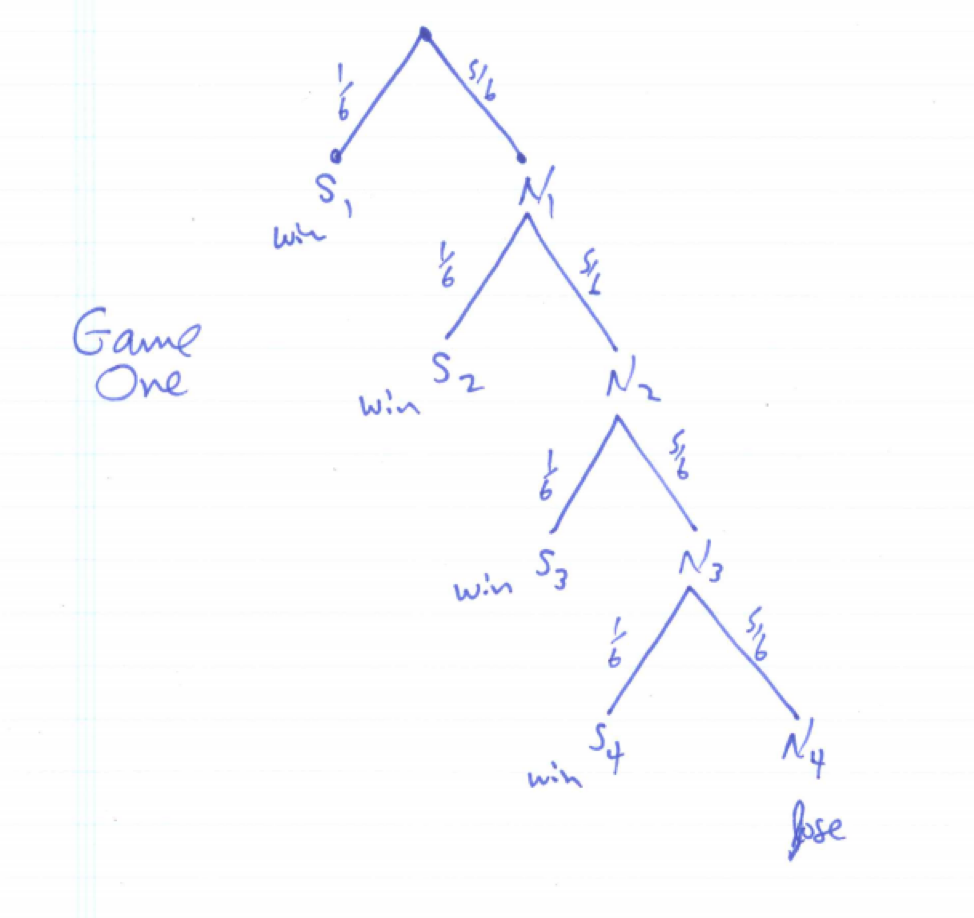
\includegraphics[width=0.3\linewidth]{01-basics-figures/chevalier_game_one} 

}

\caption{Tree Diagram for Game One}\label{fig:nice-fig-63}
\end{figure}

The tree diagram for four tosses of a die considering the two outcomes
of success or failure of getting a six on each toss generates sixteen
branches through the tree but only five branches if we terminate the
tree whenever we get a success. These branches are not equally likely,
though, so we need to be careful about calculating probabilities. When
finding the probability of at least one success in an experiment like
this we often utilize the Complement Rule because while there are many
branches that end in a success there is only one branch of all failures
so this one would be easier to calculate the probability of than adding
together the other branches.

Examine the tree diagram above and identify the one branch in the sample
space in which the gambler loses by shading it and find the probability
of this occurrence.

\[P(no \ sixes \ in \ four \ tosses)=P(S_{1}^{c} \ and \ S_{2}^{c} \ and \ S_{3}^{c} \ and \ S_{4}^{c}) = \\ P(S_{1}^{c}) \cdot P(S_{2}^{c}) \cdot P(S_{3}^{c}) \cdot P(S_{4}^{c})=(5/6)^{4}\]
Thus, by the Complement Principle,

\[P(at \ least \ one \ six \ in \ four \ tosses) = 1 - P(no \ sixes \ in \ four \ tosses) = \\ 1 - (5/6)^{4}\]

\subsection{Practice}\label{practice-2}

Are the probabilities you have found for losing or winning Game One
consistent with the Chevalier de Mere's observation that he found Game
One to be a favorable game? Explain.

\section{Analyzing Game Two}\label{analyzing_game_two}

Recall, in this game the gambler rolls a pair of dice and has 24 chances
to obtain double-six winning the amount bet if she does and losing the
bet if she does not obtain a double-six in 24 rolls. The Chevalier did
not like this game as much. We analyze the game here to see if his lack
of enthusiasm is justified.

Consider what a tree diagram would look like for this game. If we let
event \(D_{i}\) represent getting a double six on the \(i^{th}\) roll of
the dice and \(N_{i}\) represent its complement we can stop the
branching as a win whenever we hit a double six.

\begin{figure}

{\centering 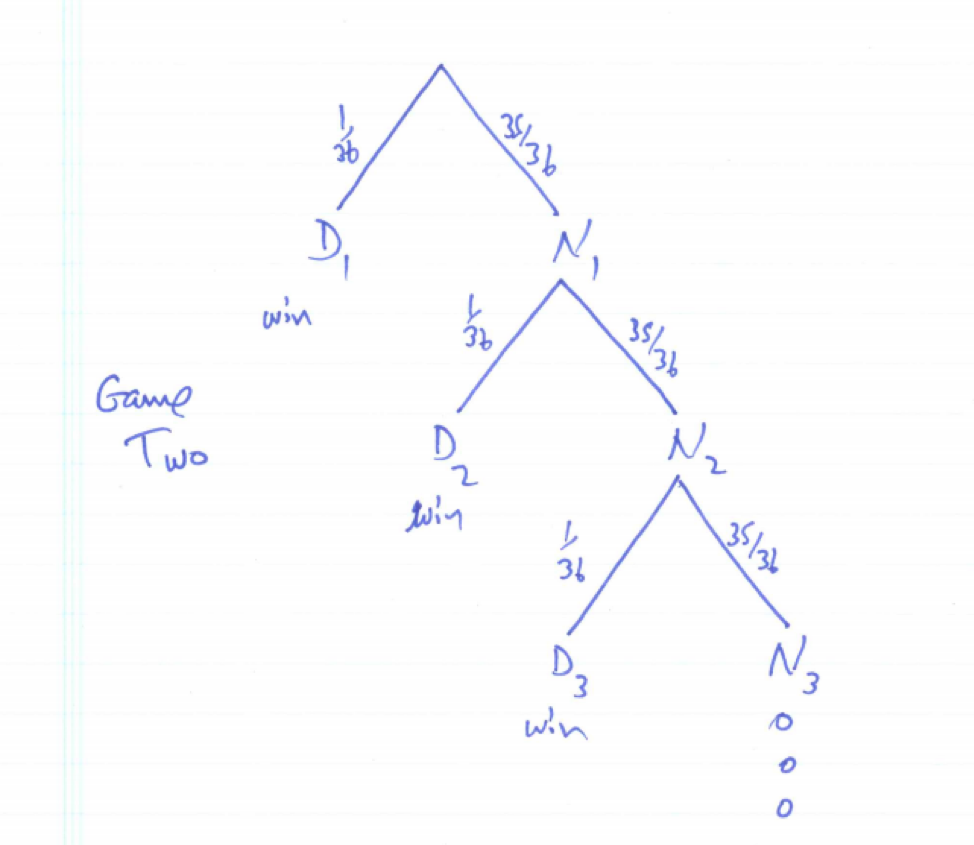
\includegraphics[width=0.3\linewidth]{01-basics-figures/chevalier_game_two} 

}

\caption{Venn Diagram of Class Composition}\label{fig:nice-fig-64}
\end{figure}

Would it be realistic to use this tree diagram to assist us find the
probability of a win? The main issue is there are so many ways to win -
on the first toss, the second toss,\ldots{}, the 24th toss. Who wants to
add up 24 separate probabilities? Maybe the complement principle can
help us since there is only one way to lose - never get a double six in
all 24 tosses. Follow the chain of reasoning:

\[P(win) = 1 - P(lose) = 1 -P(no \ sixes \ in \ 24 \ rolls) = 1 - P(N_{1} \ and \ N_{2} \ and \ ... \ N_{24}) = \\ 1 - P(N_{1}) \cdot P(N_{2}) \cdot ... \cdot P(N_{24}) = 1 - (35/36)^{24}\]

We are using the fact that the different tosses of the dice are all
independent.

\subsection{Practice}\label{practice-3}

Compare the probabilities of winning and losing Game One with the
probabilities of winning and losing Game Two and whether the opinions of
the Chevalier de Mere's games obtained through the simulation in R are
consistent with the theoretical conclusions of our probability analysis.

\section{Revisiting the Chapter Scenario - The Birthday
Problem}\label{revisiting-the-chapter-scenario---the-birthday-problem}

Given 365 days of the year (We ignore Leap Day February 29 with
apologies to the Pirate of Penzance) and only 20 people it may initially
feel like there is not much chance of a match but we are being deceived.
With our problem-solving tools of the Multiplication and Complement
Principles, we can find out for sure.

Recall The Multiplication Rule shows us that to obtain the probability
of two potentially consecutive events we multiply related probabilities:

\begin{verbatim}
$$P(A \ and \ B)= P(A) \cdot P(B \ \mid \ A)$$
If the events A and B are independent then $P(A \ and \ B)=P(A) \cdot P(B)$.
\end{verbatim}

The Complement Rule confirms that the probability of an event occurring
is one minus the probability the event does not occur:

\[P(A)= 1-P(not \ A)\] Remember, this can also be written
\(P(A)=1-P(not \ A)\).

We will build up our way into solving this problem by imagining that
individuals walk into the room one at a time and announce their birthday
to see if it matches or not with anyone else who is in the room.

When the first person walks in the room, there is no one else there so
their birthday can be any one of the 365 days without there being a
match so the probability of no match is \(365/365=1\). Suppose only this
one person is in the room. The probability that the second person to
enter the room has the different birthday is \(364/365\).

Suppose that two people are in the room and do not have the same
birthday. The probability that the third person to enter the room has a
different birthday than these two is \(363/365\).

Now, suppose three people are in the room and do not have a birthday
match. Then the probabillity that the fourth person to enter the room
has a different birthday than these three is \(362/365\).

For all of these events to occur we can use the multiplication
principle. With four people the probability of no match is
\((365/365) \cdot (364/365) \cdot (363/365) \cdot (362/365)\)

Using the complement principle for this case with four people

\[P(match)=1-P(no \ match)=1-(365/365) \cdot (364/365) \cdot (363/365) \cdot (362/365)\]

\subsection{Practice}\label{practice-4}

Extend this thinking to find the probability of no match with five
people.

We want to describe the solution in general for any number of people n
according to the tree diagram below.

\begin{figure}

{\centering 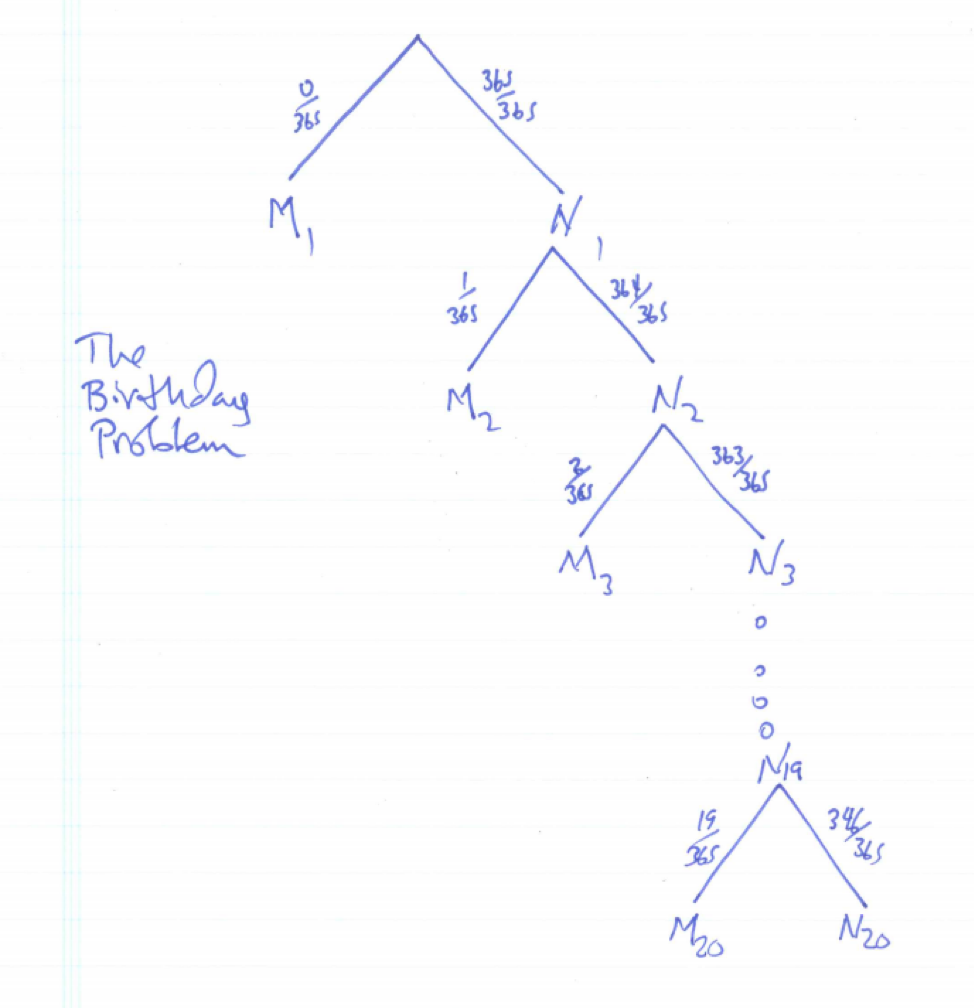
\includegraphics[width=0.3\linewidth]{01-basics-figures/birthday_problem_tree_diagram} 

}

\caption{Tree Diagram for Birthday Problem}\label{fig:nice-fig-65}
\end{figure}

A computational shortcut will help us calculate the result.

Given n people, the probability of a birthday match is

\[P(match)=1-P(no \ match)=1-\frac{365 \cdot 364 \cdot 363 \cdot ... \cdot (365-n+1)}{3655^{n}}= \\ 1-\frac{P(365,n)}{365^{n}}\]

where \(P(365,n)\) represents the permutation of 365 days taken n at a
time. We will discuss this in more detail in a later chapter.

To solve the Chapter Scenario problem, we let \(n=20\) and see

\[P(match)=1-P(no \ match)=1-\frac{P(365,20)}{365^{20}}\]

We can use the \texttt{prod()} function in R for the computation.

\begin{Shaded}
\begin{Highlighting}[]
\NormalTok{match_prob_}\DecValTok{20}\NormalTok{ <-}\StringTok{ }\DecValTok{1}\OperatorTok{-}\StringTok{ }\KeywordTok{prod}\NormalTok{(}\DecValTok{1} \OperatorTok{-}\StringTok{ }\NormalTok{(}\DecValTok{0}\OperatorTok{:}\DecValTok{19}\NormalTok{)}\OperatorTok{/}\DecValTok{365}\NormalTok{)}
\NormalTok{match_prob_}\DecValTok{20}
\end{Highlighting}
\end{Shaded}

\begin{verbatim}
## [1] 0.4114384
\end{verbatim}

So the probability of a birthday match with 20 people is 0.4114384 which
might surprise us.

\subsection{Exercise - Birthday Problem
continued}\label{exercise---birthday-problem-continued}

Continue in like fashion finding the probability of a birthday match
with 21, 22, 23, etc. people until you find the first value of n for
which this probability is greater than 0.5.

\subsection{Exercise}\label{exercise}

Suppose that a fair coin is flipped five times. What is the probability
there is at least one head?

\chapter{Conditional Probability}\label{conditional}

Conditional probability is a thing.

\section{Example one}\label{example-one}

some stuff

\section{Example two}\label{example-two}

more stuff

\chapter{Mathematical Expectation}\label{expectation}

\section{Introduction}\label{introduction}

We construct probability distributions and compute and interpret the
mathematical expectation or expected value.

\section{Chapter Scenario -
Chuck-a-Luck}\label{chapter_scenario_chuckaluck}

Chuck-A-Luck is a popular carnival game since it is easy to understand,
easy to set-up, and easy to hide when the county-mounty shows up with a
simple layout for betting as shown below. One bets on a number, one
through six. Three dice are rolled and you win the amount bet for each
time that number shows. For example, if you bet \(\$1\) on the number 5,
if that number comes up once on the three dice you win \(\$1\), if it
comes up twice you win \(\$2\), if it comes up three times you win
\(\$3\) but if it doesn't come up at all you lose \(\$1\) (or we say
your result is \(\$1\)). Is this game favorable to the players or to the
house? In the long run, how much money per game would you expect to win
or lose?

\begin{figure}

{\centering 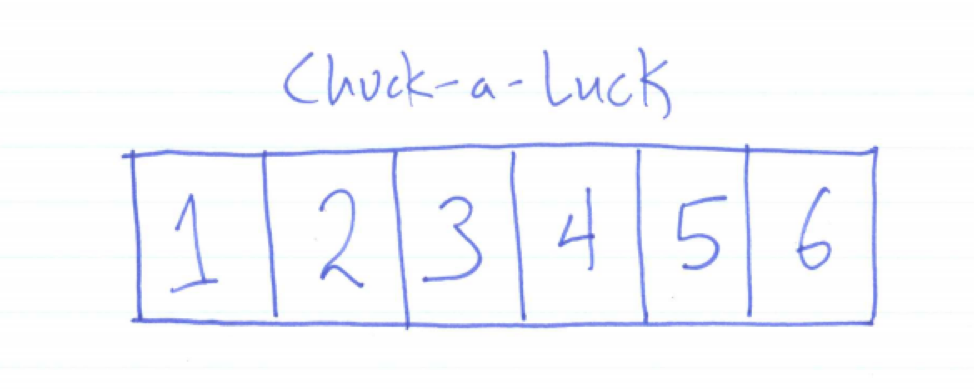
\includegraphics[width=0.3\linewidth]{01-basics-figures/chuck_a_luck_layout} 

}

\caption{Chuck-a-Luck Layout}\label{fig:nice-fig-81}
\end{figure}

\section{Example - Win Six}\label{example---win-six}

Let's start with a slightly simpler game we'll call Win Six. Suppose you
bet \(\$1\) then you roll a die. If a 1, 2, or 3 comes up you lose
\(\$1\). If a 4 or 5 comes up you win \(\$1\). If a 6 comes up you win
\(\$6\). Hey, let's call it Win Six!

Our goal is to analyze this game and determine the expected amount one
would win. We call this the mathematical expectation whic is the
theoretical mean or the weighted average of the outcomes weighted by
their probabilities. We first want to describe the \textbf{probability
distribution}, or the complete description of the different outcomes X
and their associated probabilities, P(X).

\begin{itemize}
\tightlist
\item
  X P(X)
\item
  -1 3/6
\item
  1 2/6
\item
  6 1/6
\end{itemize}

We get the mean/expected value by summing up the X times P(X)
quantities. In formula form we say

\[Mean = \sum_{x} x \cdot P(x)\]

We can determine this manually by adding the following column to the
probability distribution and summing it.

\begin{itemize}
\tightlist
\item
  X P(X) XP(X)
\item
  -1 3/6 -3/6
\item
  1 2/6 2/6
\item
  6 1/6 6/6
\end{itemize}

Sum = 5/6 = 0.833

Thus, the expected value for the game Win Six is \(+\$0.83\). Note,
since this number is positive that means this game is in the player's
favor. (One reason you will not find this game in any casino!)

\section{Chapter Scenario Revisited -
Chuck-a-Luck}\label{chapter_scenario_revisited_chuckaluck}

Recall that in the game of Chuck-a-Luck, three dice are rolled and you
win the amount bet for each time that number shows. Let's assume \(\$1\)
is bet and, without loss of generality, let's assume we bet on the
number 5. Using F to represent getting a 5 and N to represent not
getting a five and using subscripts to denote the first, second, and
third die yields the tree diagram below.

\begin{figure}

{\centering 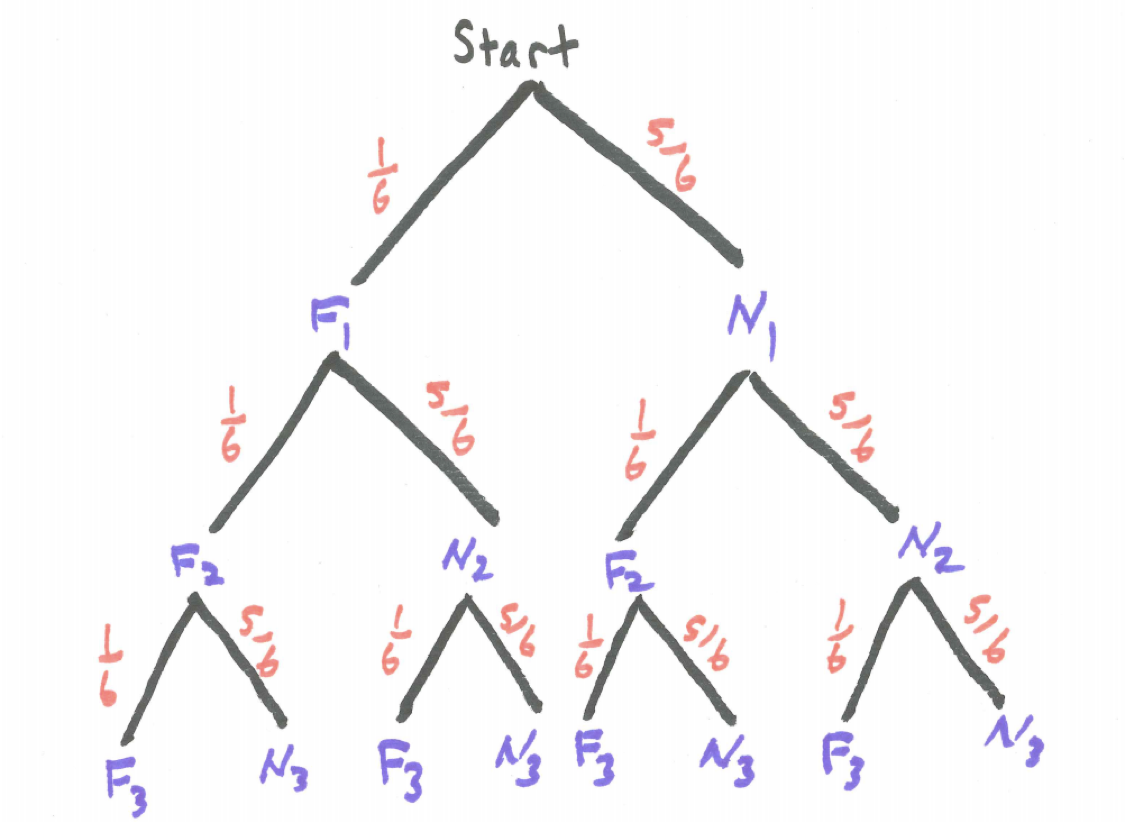
\includegraphics[width=0.3\linewidth]{01-basics-figures/chuck_a_luck_tree_diagram} 

}

\caption{Chuck-a-Luck Tree Diagram}\label{fig:nice-fig-82}
\end{figure}

Thus, \(P(0 \ fives) = (5/6)^{3}\). There are three different branches
where the result is exactly one five thus,
\(P(1 \ five) = 3 \cdot (1/6) \cdot (5/6)^{2}\). Similarly, three
brances for exactly two fives so
\(P(2 \ fives) = 3 \cdot (1/6)^{2} \cdot (5/6)\). Lastly, for three
fives, \$P(3 ~fives) = (1/6)\^{}\{3\}.

If we let X represent the winnings in these circumstances we can write
the probability distribution for X:

\begin{itemize}
\tightlist
\item
  X P(X)
\item
  -1 125/216
\item
  +1 75/216
\item
  +2 15/216
\item
  +3 1/216
\end{itemize}

Calculating the mean/expected value shows

\[Mean=\sum_{x} x \cdot P(x)= \\(-1) \cdot (125/216)+1 \cdot (75/216) +2 \cdot (15/216)+3 \cdot (1/216)=-17/216 \]

\section{Exercises}\label{exercises}

\subsection{Exercise - Slot Machine}\label{exercise---slot-machine}

Consider a dollar slot machine with three wheels each containing ten
symbols. On each wheel there is one JACKPOT symbol and nine other
non-jackpot symbols. You put \$1 in the slot and the payoffs are as
follows:

\begin{itemize}
\tightlist
\item
  If 3 JACKPOT symbols appear \$487 is returned.
\item
  If 2 JACKPOT symbols appear \$10 is returned.
\item
  If 1 JACKPOT symbol appears \$1 is returned.
\end{itemize}

Find the expected value. Note, with slot machines you put in your
\(\$1\) so you start out \(-\$1\). Make sure you take this into account
in your calculations.

\subsection{Exercise - Fair
Chuck-a-Luck}\label{exercise---fair-chuck-a-luck}

In the game of Chuck-a-Luck, if the \(\$1\) payoff was increased to some
higher payoff of d dollars per occurrence of the chosen number (so d for
one occurrence, 2d dollars for two occurrences, and 3d dollars for three
occurrences) find the value for d that would make the game fair (that
is, make the expected value 0).

\subsection{Exercise - Chuck-a-Luck Big
Prize}\label{exercise---chuck-a-luck-big-prize}

In the game of Chuck-a-Luck, if the payoff remained \(\$1\) for the
first occurrence of the chosen number and \(\$2\) for two occurrences
but changed to b dollars for three occurrences, find the value for b
that would make the game fair (that is, make the expected value 0).

\subsection{Exercise - St.~Petersburg
Paradox}\label{exercise---st.petersburg-paradox}

Here's a game for you. You flip a coin. If it comes up tails on the
first flip you win \$1. If it comes up heads on the first flip then
tails you win \$2. If it comes up heads on the first two flips then
tails you win \$4. If it comes up heads on the first three flips then
tails you win \$8. And so on. For example, if the first n flips are
heads and the next one tails then you win 2n dollars. How much would you
be willing to pay to play this game? Buffon played 2084 games. His
winnings for those games would have been \$10,057. Thus, what would you
estimate the mathematical expectation to be based on his data? Now,
complete the table below to calculate the mathematical expectaton. Does
this answer sound reasonable to you? How does this theoretical
probability match up with relative frequency.

\begin{figure}

{\centering 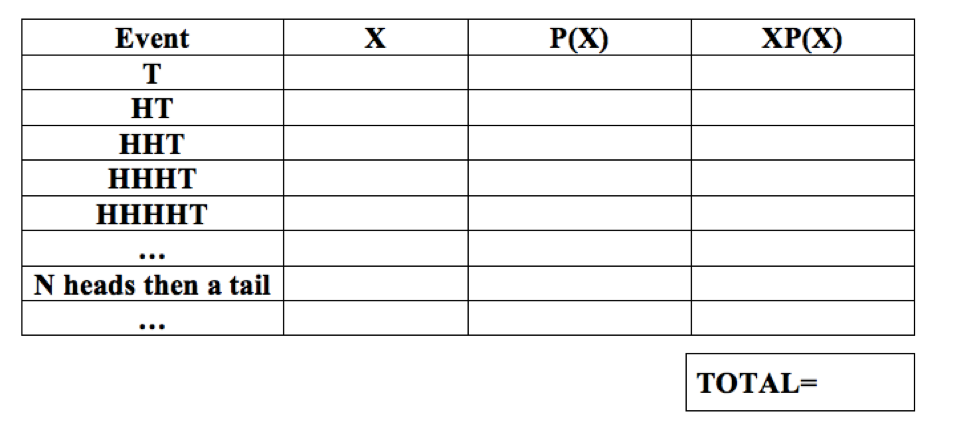
\includegraphics[width=0.3\linewidth]{01-basics-figures/st_petersburg_table} 

}

\caption{St. Petersburg Paradox Probability Distribution Table}\label{fig:nice-fig-83}
\end{figure}

\chapter{Permutations}\label{permutations}

\section{Introduction}\label{introduction}

Determine correct probabilities relies heavily on correct counting.
Combinatorics is the mathematics of counting and in this chapter we
learn how to count ordered arranements (permutations) and unordered
collections (combinations) for the ultimate purpose of tracking the
probabilities of repeated events.

\section{Chapter Scenario - GATC}\label{chapter_scenario}

\section{Permutations}\label{permutations}

Permutations are ordered arrangements. If we are given n distinct
objects and are to select k of them and place them in order, we call
this the permutation of k objects taken from n and symbolize it as
P(n,k). By looking at some examples we will determine how to calculate
permutations.

One key to calculating permutations is using the Fundamental Principle
of Counting.

\section{Fundamental Counting Principle
Principle}\label{fundamental_counting_principle}

Consider a multi-step process requiring k steps. If Step1 can be done
\(n_{1}\) ways, Step2 done \$n\_\{2\} ways, and so on up to Step k being
done \$n\_\{k\} ways, then the total number of ways the entire process
can be done \(n_{1} \cdot n_{2} \cdot ... \cdot n_{k}\) ways.

Suppose you are playing scrabble and have four distinct letters, say A,
S, N, and P. Not all of rearrangements are real words, of course, but
how many total rearrangements of these four letters would we need to
consider to check all the possible permuations? A tree diagram helps and
shows there are 24 different orderings. Using the FPC there are four
choices for the first letter, three for the second, two for the third,
and only one choice left for the last letter making the total
\(4 \cdot 3 \cdot 2 \cdot 1=4!=24\). Thus, \(P(4,4)=4!=24\).

Suppose you have seven distinct letters and you want to identify how
many four-letter strings could be made. Using the Fundamental Counting
Principle there are seven choices for the first letter, six for the
second, and so on for a total of \(P(7,4)=7 \cdot 6 \cdot 5 \cdot 4\)
which is the same as \(7!/3!\). We describe this as a general formula
below.

\section{Permutation Formula}\label{permutation-formula}

The number of orderings of k objects taken from n distinct objects is
\(P(n,k)=n!/(n-k)!=n \cdot (n-1) \cdot (n-2) \cdot ... \cdot (n-k+1)\).

\section{Example - The Line-up}\label{example---the-line-up}

Suppose that members of our class, all 20 of you, are to be seated in a
row. How many ways can this be done? Ordering 20 people selected from 20
people is \(P(20,20)=20!/0!=20!\).

What if Alice and Bob refuse to sit beside one another? Using the
Complement Principle, let's force them to sit together, count this, and
subtract from the total. Think of putting a rubberband around them then
we have only 19 things to order which can be done \(19!\) ways and then
there are 2 orders for Alice and Bob so seating orders with them
together is \(2! \cdot 19!\). Putting this together

\[(\text{# of ways with Alice and Bob apart}) = \\ 
(\text{Total}) - (\text{# of ways with Alice and Bob together}) = \\
20! - 2! \cdot 19!\]

What if there are 10 men and 10 women and we want no two men sitting
together and no two women sitting together? Suppose we start with a man.
Then alternating sex and using the Fundamental Counting Principle we see
this can be done
\(10 \cdot 10 \cdot 9 \cdot 9 \cdot 8 \cdot ... \cdot 1 \cdot 1 = 10! \cdot 10!\).
Since we could start either with a man or with a women, two choices, the
total is \(2 \cdot 10! \cdot 10!\).

\section{Example - The MISSISSIPPI
Problem}\label{example_the_mississippi_problem}

How many arrangments are there of the word MISSISSIPPI? The issue we
need to deal with is the repeated letters - there are four S's, four
I's, and two P's. If the word was LUMBERJACKS the answer would be
\(11!\) because all the letters are unique.

Let's tackle a smaller problem, learn from it, and then ramp it up.
Consider the word MISS. If the letters were all unique it would be
\(4!\) orderings but in reality there are only twelve. To see why
pretend we could tell the P's apart with color or subscripts. Then each
unique ordering of \(MISS\) is duplicated in the orderings of
\(MIS_{1}S_{2}\) because of the \(2!\) orderings of the S's. So, the
total orderings of \(MISS\) is \(4!/2!\).

Orderings of \(MISSI\) has to account for two S's and two I's so there
are a total of \(5!/(2! \cdot 2!)\).

Orderings of \(MISSISS\) has to account for four S's and two I's.
Imagining subscrips of four S's would yield \(4!\) orderings. Taking
care of everything, the total orderings of \(MISSISS\) is
\(7!/(4! \cdot 2!)\).

Tackling MISSISSIPPI, the total number of orderings is
\(11!/(4! \cdot 4! \cdot 2!)\).

\section{Exercises}\label{exercises}

\section{Exercises - Scrabble}\label{exercises---scrabble}

If you have six unique letters, how many total orderings are there of
those six letters? How many total orderings are there including those
not using all six letters?

\subsection{Exercise - The Name Game}\label{exercise---the-name-game}

Find the number of possible rearrangements for the following names -
JON, BRAN, TYRION, TORMUND, KERMIT, ARYA, SANSA, JOFFREY, ELLARIA,
CERSEI, EDDARD, LITTLEFINGER, DAENERYS TARGARYEN (as one word), DAENERYS
TARGARYEN (as two words keeping first name letters together and last
name letters together).

\subsection{Exercise - License Plates}\label{exercise---license-plates}

\begin{figure}

{\centering 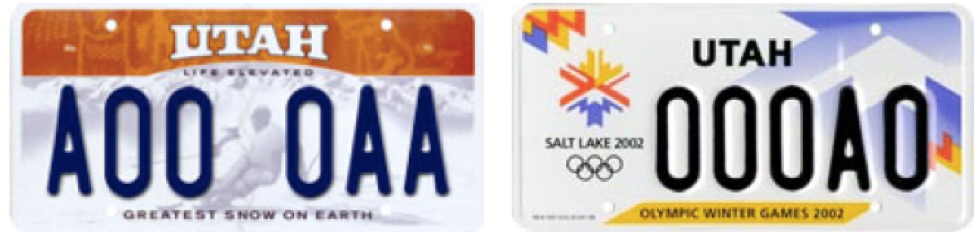
\includegraphics[width=0.3\linewidth]{01-basics-figures/utah_license_plates} 

}

\caption{Utah License Plates}\label{fig:nice-fig-91}
\end{figure}

How many different license plates are there? See if you can determine
the total number of license plates under the following schemes.

\begin{enumerate}
\def\labelenumi{(\alph{enumi})}
\item
  Life Elevated Skier or Arches This plate contains six characters,
  consisting of one letter followed by three numbers followed by two
  letters.
\item
  Olympic This plate was issued to commemorate the 2002 Olympic Winter
  Games held in Salt Lake City. As of July 1, 2002.It consists of three
  numbers followed by a letter followed by a number.
\item
  Personalized Standard Life Elevated Skier or Arches plates For Utah
  personalized license plates, the type of plate requested limits the
  number of characters that may be used on the plate, with the Life
  Elevated Skier or Arches plates allowing up to seven characters which
  may be either numbers or letters.
\item
  Personalized Motorcycle Plates These plates allow up to four
  characters which may be numbers or letters.
\end{enumerate}

\subsection{Exercise - Facts about
Permutions}\label{exercise---facts-about-permutions}

\begin{enumerate}
\def\labelenumi{(\alph{enumi})}
\tightlist
\item
  What does P(n,1) equal for all \(n \geq 1\)?
\item
  What does P(n,n) equal for all \(n \geq 1\)?
\item
  What is the relationship between P(n,n-1) and P(n,n)?
\end{enumerate}

\chapter{Combinations}\label{combinations}

\section{Introduction}\label{introduction}

While permutations count ordered arrangements, combinations are
unordered collections of items.

\section{Chapter Scenario - Three Counting Problems and an Algebra
Problem}\label{chapter_scenario_three_counting_problems}

Below are three counting problems and one algebra problem. On the
surface these appear to be unrelated problems but can you find a deep
connection between them? It might help to team up with classmates to
gain multiple perspectives.

Problem 1: Write down all the possible birth orderings for a family of
three boys and two girls (for example, BGBBG is one of them).

Problem 2: Find the number of ways that you can walk along the blocks
from point A to point B by a path of shortest length.

\begin{figure}

{\centering 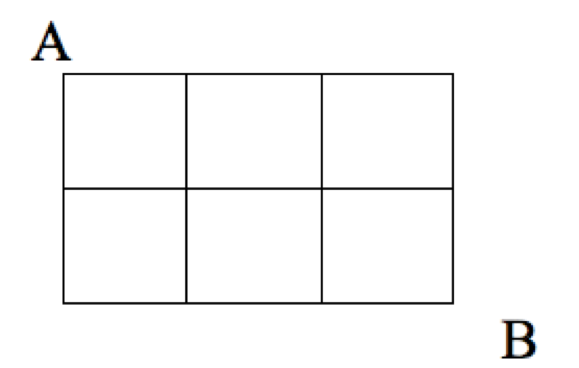
\includegraphics[width=0.3\linewidth]{01-basics-figures/block_walking_scenario} 

}

\caption{Block-walking Scenario}\label{fig:nice-fig-101}
\end{figure}

Problem 3: How many ways could two captains be chosen from the five
starting members of a basketball team?

Problem 4: Expand the following: \((p + q)^{5}\).

\section{Example - From Class Line-up to Class
Committee}\label{example_class_lineup_to_class_committee}

If we were to select four people from our class of 20 and line them up,
this could be done \(P(20,4)=20!/16!=20 \cdot 19 \cdot 18 \cdot 17\)
ways. But if we are interested in the number of unordered committees of
four rather than ordered line-ups we notice that for each selection of
four people, there were \(4!=4 \cdot 3 \cdot 2 \cdot 1\) line-ups
counted so the number of unordered committees is
\((20 \cdot 19 \cdot 18 \cdot 17)/(4 \cdot 3 \cdot 2 \cdot 1)\).

We call an undordered collection of k objects selected from n distinct
objects a combination and use the notation \(\dbinom{n}{k}\). A simple
way to think of this is to find the permutation of k objects selected
from n objects, \(P(n,k)=n!/(n-k)!\) and divide out the order, \(k!\).
Putting all this together we get the following formula.

\section{Combination Formula}\label{combination-formula}

The number of unordered collections of k objects selected from n
distinct objects is

\[\dbinom{n}{k}=\frac{P(n,k)}{k!}=\frac{n!}{(n-k)!k!}=
\frac{n(n-1)(n-2)...(n-k+1)}{k(k-1)(k-2)...3 \cdot 2 \cdot 1}\]

Using this notation to recap the number of unordered committees selected
from 20 students we see

\[\dbinom{20}{4}=\frac{20!}{16! \cdot 4!}=\frac{20 \cdot 19 \cdot 18 \cdot 17}{4 \cdot 3 \cdot 2 \cdot 1}\]

\section{Exercises}\label{exercises}

\subsection{Exercise - Alphabet}\label{exercise---alphabet}

Consider the 26 letters in our alphabet.

\begin{enumerate}
\def\labelenumi{(\alph{enumi})}
\item
  How many different three letter strings can we make if repetition of
  letters is allowed?
\item
  How many different three letter strings can we make if repetition of
  letters is not allowed?
\item
  How many ways could three different letters be chosen?
\end{enumerate}

\subsection{Exercise - Facts about
Combinations}\label{exercise---facts-about-combinations}

\begin{enumerate}
\def\labelenumi{(\alph{enumi})}
\tightlist
\item
  What is \(\dbinom{n}{0}\) for all \(n \geq 1\)?
\item
  What is \(\dbinom{n}{1}\) for all \(n \geq 1\)?
\item
  What is \(\dbinom{n}{n}\) for all \(n \geq 1\)?
\item
  What is the relationship between \(\dbinom{n}{k}\) and
  \(\dbinom{n}{n-k}\)?
\end{enumerate}

\chapter{The Binomial Distribution}\label{the-binomial-distribution}

We describe some cool stuff about the Binomial Distribution in this
chapter.

\chapter{Normal Distribution}\label{normal}

Not everything is Normal (we certainly aren't), but it's useful!

\chapter{Multinomial Distribution}\label{multinom}

Beyond the Binomial to the Multinomial\ldots{}

\chapter{Fancier Distributions}\label{fancy}

Oooh, fancy!

\chapter{Bayes Theorem}\label{bayes}

Probability can give you (apparent) superpowers!

\chapter{Genetics}\label{genetics}

Placeholder chapter for draft genetics content

\section{Appendix 1: Genetics
Examples}\label{appendix-1-genetics-examples}

In this appendix, you are introduced to the absolute basic terminology
of genetics and how the principles of probability that you learned in
chapter 1 can be applied to genetics.\\
We are going to adapt the examples from the main part of chapter 1 to
genetics. We'll look at some of the same tree diagrams and simulations
but within a simple genetics framework (rather than coin flips and
urns).

\subsection{Genetics Terminology}\label{genetics-terminology}

For now, we are going to use the minimum of genetic lingo to get going:

\textbf{trait}: a characteristic, something you can see or measure
(e.g.~height, Huntington's disease)

\textbf{gene}: the DNA that controls a trait (e.g.~hemoglobin beta gene)
usually shown with a letter or letters (e.g.~Hb)

\textbf{variant}: one of several versions of a gene (e.g.~HbS variant in
hemoglobin beta that can cause Sickle Cell Anemia but there are other
variants of the same gene (HbC, HbE, etc.), a.k.a. allele)

\textbf{chromosome}: long, continuous stretch of DNA that contains many
genes (humans have 2 copies of each of 22 numbered chromosomes and
either 2 X chromosomes for females or an X and a Y for males)

\textbf{gamete}: specialized cell that has only 1 copy of each
chromosome that is used during sexual reproduction (e.g.~egg or sperm)

\subsection{Genetics Basics}\label{genetics-basics}

\subsubsection{intro to chromosomal
genetics}\label{intro-to-chromosomal-genetics}

\begin{itemize}
\tightlist
\item
  humans have 2 copies of every gene (can be same variant or different)
\item
  \textbf{meiosis} is the process of making gametes with only 1 copy of
  all of the genes
\item
  \textbf{fertilization} fuses two gametes each with 1 copy back into a
  cell/organism with 2 copies (1 from each parent/gamete)
\end{itemize}

To summarize the important points about \textbf{meiosis}, parents each
make gametes that contain only one of their 2 possible copies of each
chromosome. Then the gametes can fuse together by fertilization to make
the offspring (next generation) that again has 2 copies of each
chromosome (one from each of their parents).

Below are some cartoons of meiosis starting with an example cell that
has 2 chromosomes (one with the A gene and a second with the B gene) and
this organism has 2 copies of each chromosome.

\begin{figure}

{\centering 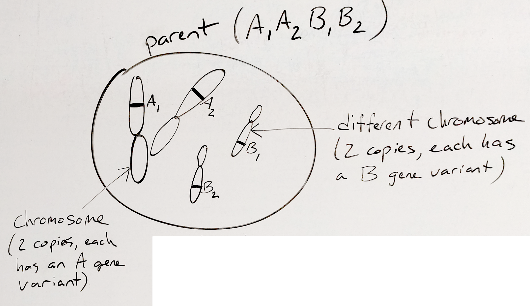
\includegraphics[width=0.75\linewidth]{01-basics-figures/meiosis1} 

}

\caption{cartoon example cell}\label{fig:gen-fig-151}
\end{figure}

Notice that the chromosomes have different variants.

When that cell goes through meiosis, it produces gametes that have one
copy of each of the 2 different chromosomes.

\begin{figure}

{\centering 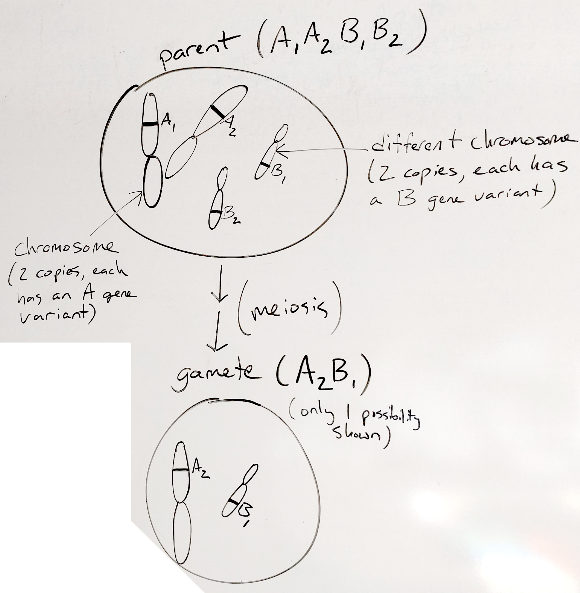
\includegraphics[width=0.75\linewidth]{01-basics-figures/meiosis2} 

}

\caption{making gametes}\label{fig:gen-fig-152}
\end{figure}

Compare the original/parent and gamete and convince yourself that this
gamete has one of each of the different chromosomes in the
original/parent organism. Notice that the figure below says that the
gamete shown is only one of the possibilities. If you like to think
ahead, what are the other possibilities? If you're not up for it yet,
don't worry, we'll get there.

To make an offspring, 2 gametes fuse by fertilization.

\begin{figure}

{\centering 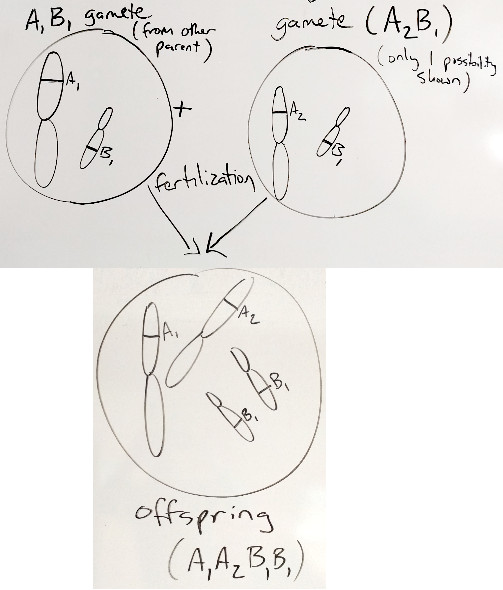
\includegraphics[width=0.75\linewidth]{01-basics-figures/meiosis3} 

}

\caption{fertilization}\label{fig:gen-fig-153}
\end{figure}

Since each gamete has only 1 copy of each chromosome, when 2 gametes
fuse, there are again 2 copies of each chromosome (one from each of
their parents). So, new humans have 2 chromosomes, one from each parent.

\subsubsection{thinking
probilitisically}\label{thinking-probilitisically}

To wrap this back around to probability and tree diagrams, you can think
of each parent as having a coin for each chromosome, and each
chromosome-coin has 2 sides - H and T for a coin, one for each copy of
the chromosome (A1 or A2). The chromosome version is equally likely to
fall on the A1 or A2 ``side'' (as long as we only consider one gene on
each chromosome, which we will do for now). So, our tree diagram looks
like this:

\begin{figure}

{\centering 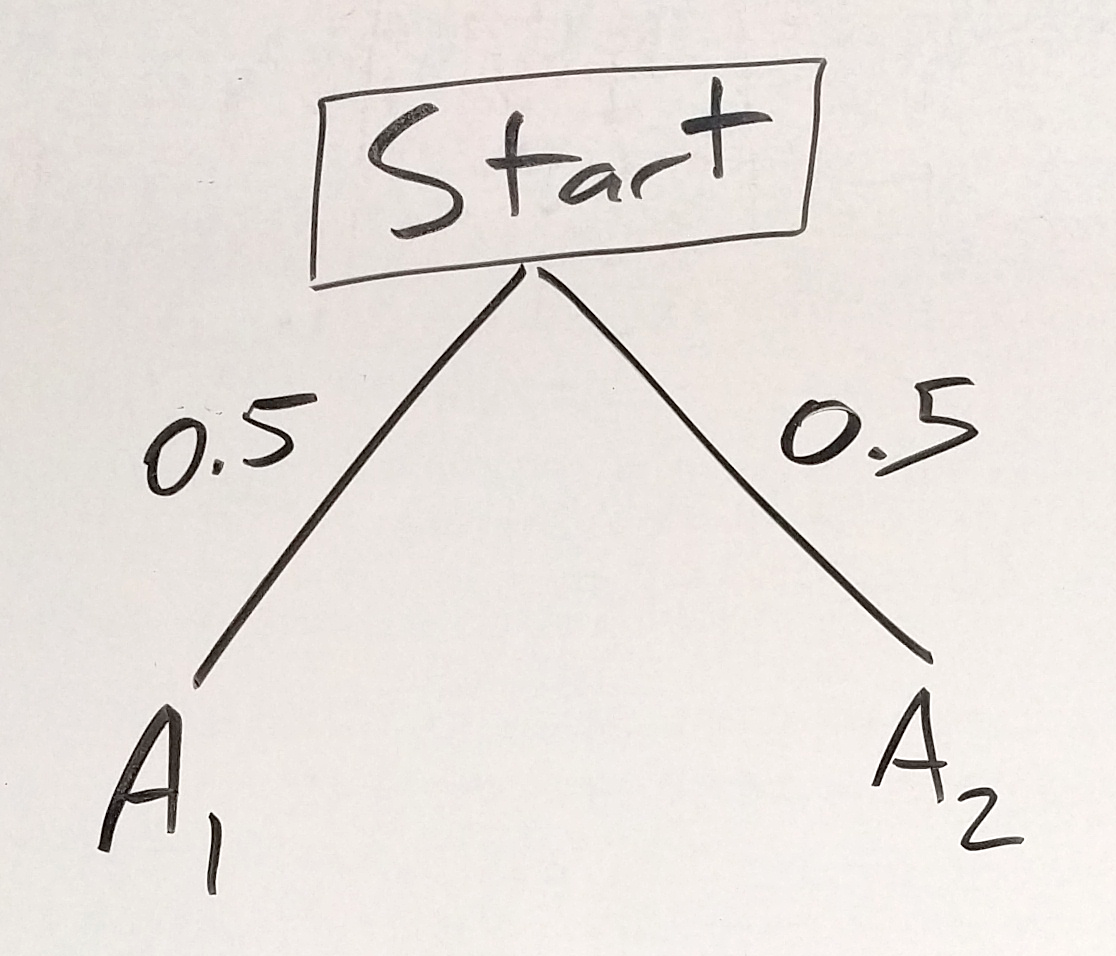
\includegraphics[width=0.5\linewidth]{01-basics-figures/1csome_tree} 

}

\caption{one chromosome tree - first parent}\label{fig:gen-fig-154}
\end{figure}

Now if we think of the gametes from the second parent as a second
``coin'' with A1 and A2 ``sides'', our tree diagram looks like this:

\begin{figure}

{\centering \includegraphics[width=0.7\linewidth]{01-basics-figures/1csome_tree2} 

}

\caption{one chromosome tree - second parent}\label{fig:gen-fig-155}
\end{figure}

Then we can use the multiplication rule to find the probabilities of the
different offspring as seen below:

\begin{figure}

{\centering \includegraphics[width=0.9\linewidth]{01-basics-figures/1csome_tree3} 

}

\caption{one chromosome tree - offspring}\label{fig:gen-fig-156}
\end{figure}

We can also use the addition rule to clean up our prediction a bit since
most of the time it doesn't matter which parent you get an allele from,
so A1A2 and A2A1 are equivalent and we can add their probabilities
together to get a combined \(p(A1A2)=0.5\).

Also notice that in the tree diagrams and in parentheses in the meiosis
drawings that we often just write the gene/variant shorthand. This
shorthand is called the \textbf{genotype} and is pretty useful since it
can save you from drawing a lot of chromosomes, but if you need the
chromosomes to be sure you understand what's going on, feel free to
sketch away.

\subsubsection{intro to DNA}\label{intro-to-dna}

There are 4 main DNA letters (a.k.a. \emph{bases}) - A, T, C, G - that
make up genes, which can be thought of as DNA ``words''. While it's not
my favorite analogy, it works reasonably well - genes are collections of
DNA information. There are variants (different versions) of genes that
change the letters, and many of those change the information the gene
contains, and can change the organism.

\subsubsection{\texorpdfstring{genetic
``notation''}{genetic notation}}\label{genetic-notation}

Geneticists (a lot like mathematicians) use abbreviations as short cuts
a lot. They are first introduced above in the \emph{Genetics
Terminology} section, and again discussed at the end of the
\emph{Thinking Probabilistically} section but we'll lay it out more
here.

Every gene has an abbreviated name (like a nickname) that makes it
easier to write. For example, the hemoglobin beta gene goes by
\textbf{Hb}. We use that as a base, then we add other letters to modify
this name to show that we are talking about specific variants like the
\textbf{HbS} variant in hemoglobin beta that can cause sickle cell
anemia. Just to break that down, the \textbf{Hb} part tells us the gene,
and the \textbf{S} part tells us which variant.

Sometimes we will use numbers, such as A1 and A2 to mean the 1 and 2
variants of the A gene, or for other genes we'll use lowercase and
uppercase, such as B and b, to mean different variants of the same gene.

And as a review, writing just the letter shorthand for all of the genes
and variants together is the \textbf{genotype} of an organism.

\subsection{Genetics Simulation}\label{genetics-simulation}

Now we'll use R to simulate the same situation shown in the tree diagram
above. This version takes the long way around, but it conceptually
models meiosis (gamete formation) and fertilization for 1000 offspring.

Our first set of parents have the genotypes below:\\
parent 1: A1/A1\\
parent 2: A2/A2

The code below simulates meiosis and fertilization of 1000 offspring,
makes a table, and graphs the results.

\begin{Shaded}
\begin{Highlighting}[]
\CommentTok{# set up the different variants that each parent has}
\NormalTok{parent1_variants <-}\StringTok{ }\KeywordTok{c}\NormalTok{(}\StringTok{'A1'}\NormalTok{,}\StringTok{'A1'}\NormalTok{)}
\NormalTok{parent2_variants <-}\StringTok{ }\KeywordTok{c}\NormalTok{(}\StringTok{'A2'}\NormalTok{,}\StringTok{'A2'}\NormalTok{)}

\CommentTok{# list of 1000 gametes from each parent, probability of each is equal by default}
\NormalTok{parent1_gametes <-}\StringTok{ }\KeywordTok{sample}\NormalTok{(parent1_variants, }\DecValTok{1000}\NormalTok{, }\DataTypeTok{replace =} \OtherTok{TRUE}\NormalTok{)}
\NormalTok{parent2_gametes <-}\StringTok{ }\KeywordTok{sample}\NormalTok{(parent2_variants, }\DecValTok{1000}\NormalTok{, }\DataTypeTok{replace =} \OtherTok{TRUE}\NormalTok{)}

\CommentTok{# put gametes together to make 1000 offspring}
\NormalTok{cross_x1 <-}\StringTok{ }\KeywordTok{paste}\NormalTok{(parent1_gametes, parent2_gametes, }\DataTypeTok{sep=}\StringTok{"/"}\NormalTok{)}
\NormalTok{offspring1 <-}\StringTok{ }\KeywordTok{data.frame}\NormalTok{(}\KeywordTok{table}\NormalTok{(cross_x1))}

\CommentTok{# table}
\NormalTok{knitr}\OperatorTok{::}\KeywordTok{kable}\NormalTok{(offspring1, }\DataTypeTok{caption =} \StringTok{'A1xA2 parent cross simulation'}\NormalTok{, }\DataTypeTok{booktabs =} \OtherTok{TRUE}\NormalTok{)}
\end{Highlighting}
\end{Shaded}

\begin{table}

\caption{\label{tab:unnamed-chunk-10}A1xA2 parent cross simulation}
\centering
\begin{tabular}[t]{lr}
\toprule
cross\_x1 & Freq\\
\midrule
A1/A2 & 1000\\
\bottomrule
\end{tabular}
\end{table}

\begin{Shaded}
\begin{Highlighting}[]
\CommentTok{# makes a bar graph of the frequency of genotypes}
\KeywordTok{ggplot}\NormalTok{(offspring1, }\KeywordTok{aes}\NormalTok{(}\DataTypeTok{x=}\NormalTok{cross_x1, }\DataTypeTok{y=}\NormalTok{Freq)) }\OperatorTok{+}\StringTok{ }\KeywordTok{geom_bar}\NormalTok{(}\DataTypeTok{stat=}\StringTok{"identity"}\NormalTok{)}
\end{Highlighting}
\end{Shaded}

\includegraphics{probriskreward-bookdown_files/figure-latex/unnamed-chunk-10-1.pdf}

Now that we have the results for that set of offspring (all have the
A1/A2 genotype), we can look at these offspring as parents for a new
generation of offspring. Now the parents are:\\
parent 1: A1/A2\\
parent 2: A1/A2

The code below simulates meiosis and fertilization of 1000 offspring,
makes a table, and graphs the results.

\begin{Shaded}
\begin{Highlighting}[]
\CommentTok{# set up the different variants that each parent has}
\NormalTok{parent3_variants <-}\StringTok{ }\KeywordTok{c}\NormalTok{(}\StringTok{'A1'}\NormalTok{,}\StringTok{'A2'}\NormalTok{)}
\NormalTok{parent4_variants <-}\StringTok{ }\KeywordTok{c}\NormalTok{(}\StringTok{'A1'}\NormalTok{,}\StringTok{'A2'}\NormalTok{)}

\CommentTok{# list of 1000 gametes from each parent, probability of each is equal by default}
\NormalTok{parent3_gametes <-}\StringTok{ }\KeywordTok{sample}\NormalTok{(parent3_variants, }\DecValTok{1000}\NormalTok{, }\DataTypeTok{replace =} \OtherTok{TRUE}\NormalTok{)}
\NormalTok{parent4_gametes <-}\StringTok{ }\KeywordTok{sample}\NormalTok{(parent4_variants, }\DecValTok{1000}\NormalTok{, }\DataTypeTok{replace =} \OtherTok{TRUE}\NormalTok{)}

\CommentTok{# put gametes together to make 1000 offspring}
\NormalTok{cross_x2 <-}\StringTok{ }\KeywordTok{paste}\NormalTok{(parent3_gametes, parent4_gametes, }\DataTypeTok{sep=}\StringTok{"/"}\NormalTok{)}
\NormalTok{cross_x2 <-}\StringTok{ }\KeywordTok{gsub}\NormalTok{(}\StringTok{"A2/A1"}\NormalTok{, }\StringTok{"A1/A2"}\NormalTok{, cross_x2) }\CommentTok{# order doesn't matter}
\NormalTok{offspring2 <-}\StringTok{ }\KeywordTok{data.frame}\NormalTok{(}\KeywordTok{table}\NormalTok{(cross_x2))}

\CommentTok{# table}
\NormalTok{knitr}\OperatorTok{::}\KeywordTok{kable}\NormalTok{(offspring2, }\DataTypeTok{caption =} \StringTok{'A1/A2 inter-cross simulation'}\NormalTok{, }\DataTypeTok{booktabs =} \OtherTok{TRUE}\NormalTok{)}
\end{Highlighting}
\end{Shaded}

\begin{table}

\caption{\label{tab:unnamed-chunk-11}A1/A2 inter-cross simulation}
\centering
\begin{tabular}[t]{lr}
\toprule
cross\_x2 & Freq\\
\midrule
A1/A1 & 263\\
A1/A2 & 496\\
A2/A2 & 241\\
\bottomrule
\end{tabular}
\end{table}

\begin{Shaded}
\begin{Highlighting}[]
\CommentTok{# makes a bar graph of the frequency of genotypes}
\KeywordTok{ggplot}\NormalTok{(offspring2, }\KeywordTok{aes}\NormalTok{(}\DataTypeTok{x=}\NormalTok{cross_x2, }\DataTypeTok{y=}\NormalTok{Freq)) }\OperatorTok{+}\StringTok{ }\KeywordTok{geom_bar}\NormalTok{(}\DataTypeTok{stat=}\StringTok{"identity"}\NormalTok{)}
\end{Highlighting}
\end{Shaded}

\includegraphics{probriskreward-bookdown_files/figure-latex/unnamed-chunk-11-1.pdf}

How does this compare to our predicted probabilities from the tree
diagram?\\
Remember that they were:\\
\(p(A1/A1) = 0.25\)\\
\(p(A1/A2) = 0.5\)\\
\(p(A2/A2) = 0.25\)

Should be reasonably close.

Just as an additional example, the same code adapted to use B and b
variants of the B gene:

\begin{Shaded}
\begin{Highlighting}[]
\NormalTok{parent1_variants <-}\StringTok{ }\KeywordTok{c}\NormalTok{(}\StringTok{'B'}\NormalTok{,}\StringTok{'B'}\NormalTok{)}
\NormalTok{parent2_variants <-}\StringTok{ }\KeywordTok{c}\NormalTok{(}\StringTok{'b'}\NormalTok{,}\StringTok{'b'}\NormalTok{)}

\NormalTok{parent1_gametes <-}\StringTok{ }\KeywordTok{sample}\NormalTok{(parent1_variants, }\DecValTok{1000}\NormalTok{, }\DataTypeTok{replace =} \OtherTok{TRUE}\NormalTok{)}
\NormalTok{parent2_gametes <-}\StringTok{ }\KeywordTok{sample}\NormalTok{(parent2_variants, }\DecValTok{1000}\NormalTok{, }\DataTypeTok{replace =} \OtherTok{TRUE}\NormalTok{)}

\NormalTok{cross_x1 <-}\StringTok{ }\KeywordTok{paste}\NormalTok{(parent1_gametes, parent2_gametes, }\DataTypeTok{sep=}\StringTok{""}\NormalTok{)}

\NormalTok{offspring1 <-}\StringTok{ }\KeywordTok{data.frame}\NormalTok{(}\KeywordTok{table}\NormalTok{(cross_x1))}
\NormalTok{knitr}\OperatorTok{::}\KeywordTok{kable}\NormalTok{(offspring1, }\DataTypeTok{caption =} \StringTok{'BBxbb parent cross simulation'}\NormalTok{, }\DataTypeTok{booktabs =} \OtherTok{TRUE}\NormalTok{)}
\end{Highlighting}
\end{Shaded}

\begin{table}

\caption{\label{tab:unnamed-chunk-12}BBxbb parent cross simulation}
\centering
\begin{tabular}[t]{lr}
\toprule
cross\_x1 & Freq\\
\midrule
Bb & 1000\\
\bottomrule
\end{tabular}
\end{table}

\begin{Shaded}
\begin{Highlighting}[]
\KeywordTok{ggplot}\NormalTok{(offspring1, }\KeywordTok{aes}\NormalTok{(}\DataTypeTok{x=}\NormalTok{cross_x1, }\DataTypeTok{y=}\NormalTok{Freq)) }\OperatorTok{+}\StringTok{ }\KeywordTok{geom_bar}\NormalTok{(}\DataTypeTok{stat=}\StringTok{"identity"}\NormalTok{)}
\end{Highlighting}
\end{Shaded}

\includegraphics{probriskreward-bookdown_files/figure-latex/unnamed-chunk-12-1.pdf}

Now intercross the offspring from the first cross, each is Bb:

\begin{Shaded}
\begin{Highlighting}[]
\NormalTok{parent3_variants <-}\StringTok{ }\KeywordTok{c}\NormalTok{(}\StringTok{'B'}\NormalTok{,}\StringTok{'b'}\NormalTok{)}
\NormalTok{parent4_variants <-}\StringTok{ }\KeywordTok{c}\NormalTok{(}\StringTok{'B'}\NormalTok{,}\StringTok{'b'}\NormalTok{)}

\NormalTok{parent3_gametes <-}\StringTok{ }\KeywordTok{sample}\NormalTok{(parent3_variants, }\DecValTok{1000}\NormalTok{, }\DataTypeTok{replace =} \OtherTok{TRUE}\NormalTok{)}
\NormalTok{parent4_gametes <-}\StringTok{ }\KeywordTok{sample}\NormalTok{(parent4_variants, }\DecValTok{1000}\NormalTok{, }\DataTypeTok{replace =} \OtherTok{TRUE}\NormalTok{)}

\NormalTok{cross_x2 <-}\StringTok{ }\KeywordTok{paste}\NormalTok{(parent3_gametes, parent4_gametes, }\DataTypeTok{sep=}\StringTok{""}\NormalTok{)}
\NormalTok{cross_x2 <-}\StringTok{ }\KeywordTok{gsub}\NormalTok{(}\StringTok{"bB"}\NormalTok{, }\StringTok{"Bb"}\NormalTok{, cross_x2)}
\NormalTok{offspring2 <-}\StringTok{ }\KeywordTok{data.frame}\NormalTok{(}\KeywordTok{table}\NormalTok{(cross_x2))}
\NormalTok{knitr}\OperatorTok{::}\KeywordTok{kable}\NormalTok{(offspring2, }\DataTypeTok{caption =} \StringTok{'Bb inter-cross simulation'}\NormalTok{, }\DataTypeTok{booktabs =} \OtherTok{TRUE}\NormalTok{)}
\end{Highlighting}
\end{Shaded}

\begin{table}

\caption{\label{tab:unnamed-chunk-13}Bb inter-cross simulation}
\centering
\begin{tabular}[t]{lr}
\toprule
cross\_x2 & Freq\\
\midrule
bb & 249\\
Bb & 477\\
BB & 274\\
\bottomrule
\end{tabular}
\end{table}

\begin{Shaded}
\begin{Highlighting}[]
\KeywordTok{ggplot}\NormalTok{(offspring2, }\KeywordTok{aes}\NormalTok{(}\DataTypeTok{x=}\NormalTok{cross_x2, }\DataTypeTok{y=}\NormalTok{Freq)) }\OperatorTok{+}\StringTok{ }\KeywordTok{geom_bar}\NormalTok{(}\DataTypeTok{stat=}\StringTok{"identity"}\NormalTok{)}
\end{Highlighting}
\end{Shaded}

\includegraphics{probriskreward-bookdown_files/figure-latex/unnamed-chunk-13-1.pdf}

\bibliography{book.bib,packages.bib}


\end{document}
